\documentclass[11pt]{article}
\usepackage{graphicx}
\graphicspath{{/Users/justindoty/Documents/Research/Dissertation/Production_QR_Proxy/Code/}}
\usepackage{graphics}
\usepackage{amsfonts}
\usepackage{amsmath}
\usepackage{amstext}
\usepackage{tabularx}
\usepackage{mathrsfs}
\usepackage{subfigure}
\usepackage[dvipsnames]{xcolor}
\usepackage{lscape}
\usepackage{longtable}
\usepackage{bm}
\usepackage{bbm}
\usepackage{chngcntr}
\usepackage{setspace}
\usepackage{caption}
\usepackage{float}
\usepackage{multirow}
\usepackage{booktabs}
\usepackage{natbib}
\usepackage{fancyvrb}
\usepackage{enumitem}
\usepackage[multiple]{footmisc}
\newtheorem{assump}{Assumption}[section]
\newtheorem{lemma}{Lemma}[section]
\newtheorem{theorem}{Theorem}[section]


\usepackage[multiple]{footmisc}

%Set margins and text size
\setlength{\textwidth}{6.5in} \setlength{\textheight}{8.8in}
\setlength{\topmargin}{-0.5in}
\setlength{\oddsidemargin}{-0.01in}{}
\setlength{\parskip}{1.6mm}
\parskip=.06in
{}
%Some useful short-cuts
\def\argmax{\mathop{\rm arg\,max}}
\def\argmin{\mathop{\rm arg\,min}}



\setcounter{section}{0} % starts numbering section 1start_value=[0.498,-0.2874,0.4314,0.5444];

\setcounter{page}{1}



\usepackage{hyperref}
\hypersetup{
    colorlinks=true,
    allcolors=Violet
}
\begin{document}

\title{Heterogeneity in Firms: \\
A Proxy Variable Approach for Quantile Production Functions
%\footnote{}
}

\author{Justin Doty\thanks{Department of Economics, University of Iowa, S321 Pappajohn Business Building, 21 E Market St, Iowa City, IA 52242. Email: \href{mailto:justin-doty@uiowa.edu}{\texttt{justin-doty@uiowa.edu}}} and Suyong Song\thanks{Department of Economics and Finance, University of Iowa, W360 Pappajohn Business Building, 21 E Market St, Iowa City, IA 52242. Email: \href{mailto:suyong-song@uiowa.edu}{\texttt{suyong-song@uiowa.edu}}}
}

\date {\today}
\maketitle


\begin{abstract}
We propose a new approach to estimate firm-level production functions in which output elasticities are heterogeneous across the firm-size distribution. 
This paper extends the proxy variable approach for estimating production functions to the conditional quantiles of firm production. Production function parameters are identified by both conditional mean and quantile restrictions in a two-stage approach. We show that this method allows us to capture heterogeneity in output elasticities along the firm-size distribution that may not be found in conditional mean estimates of \cite{Olley1996} and \cite{Levinsohn2003}. We provide small-sample evidence in a Monte Carlo study to show that this approach is robust compared to other production function estimators. The method is applied to firm and plant-level manufacturing data from the US, Chile, and Colombia.
\end{abstract}


\textit{Keywords:} Production functions, Heterogeneous elasticity, Nonlinear quantile regression

\textit{JEL Classification:} C14, C36, D24


\pagenumbering{arabic}

\baselineskip25pt

%\singlespacing
\onehalfspacing
%\doublespacing

\section{Introduction}

Production function estimation is an ongoing and historical empirical research topic that links firm's input to output decisions. Identification of the output elasticities and consequently the distribution of firm-level productivity is constrained by endogeneity issues. This is because productivity is unobserved by the econometrician, but observed by the firm when making input decisions. 

A popular approach to address this issue is to introduce a proxy variable such as investment, made popular by \cite{Olley1996} (OP) or an intermediate material input using \cite{Levinsohn2003} (LP) or \cite{Ackerberg2015} (ACF). These proxies are functions of a state variable such as capital and unobserved productivity. Under certain assumptions, this function is strictly increasing in its scalar unobserved productivity component. Inverting this function controls for unobserved productivity and the production function parameters can be estimated with a simple two-stage estimator.

While these methods have been useful in identifying the production function parameters and recovering consistent estimates of total factor productivity (TFP), resulting estimates may be biased if there is additional heterogeneity in production technology across firms. Thus, allowing for heterogeneous coefficients is one possible way to capture these differences. The literature on heterogeneous production functions is small relative to the empirical research using the homogeneous coefficient model, even though many empirical studies have found heterogeneity in firms behaviors and decisions.\footnote{Some notable examples are \cite*{Kasahara2015}, \cite*{balat}, \cite*{Li2017} and \cite*{mert} to name of few. Also \cite{Gandhi2020} who estimate a nonparametric production function and obtain heterogeneous estimates.} This is because estimating the homogeneous coefficient model by itself is very difficult due to the issue of unobserved productivity. 

In our approach we allow for firm heterogeneity in production technology beyond a Hick's neutral productivity shock to be driven by the rank of the unobserved ex-post production shock.  We use the proxy variable approach in this framework in order to control for the part of production unobservables that are correlated with input decisions. The literature on control function approaches for quantile regression models is relatively small so it is not straightforward to estimate production functions by allowing for endogenous inputs and their heterogeneous coefficients.\footnote{See for example \cite{Chesher2003}, \cite{Ma2006}, \cite{Lee2007} and \cite{2009a}} We are not aware of any published paper which takes into account for the endogeneity issue of production functions in the conventional quantile regression framework. We fill the gap in this paper by proposing an easy-to-implement estimator.

We show through simulation, that our proposed two-step estimator performs relatively well to the popular control function approach of \cite{Levinsohn2003} and is successful in both capturing heterogeneous output elasticities and controlling for unobserved productivity. In our empirical application, we consider several popular firm and plant-level manufacturing datasets and compare our estimator to the LP estimator. We show that heterogeneity in these estimates implies differences in other features of firm production, such as returns to scale, capital intensity and productivity.

The rest of the paper is organized as follows. Section \ref{litreview} reviews prior approaches for production function estimation and the interpretations of quantile production functions. Section \ref{ourmodel} introduces the econometric model and the proposed estimator. Section \ref{montecarlo} presents finite-sample behaviors of the estimator via Monte Carlo experiments and Section \ref{application} applies this estimator to US, Chilean, and Colombian manufacturing datasets. Section \ref{conclusion} concludes with directions for future research.

\section{Literature Review} \label{litreview}
\subsection{Production Function Estimation}

We briefly review the LP (2003) procedure for estimating a \textit{value-added} production function (in logs) \footnote{We consider a value-added production function here to be consistent with the model we introduce in Section \ref{ourmodel}}.

\begin{equation}
y_{it}=(\beta_{0}+\omega_{it})+\beta_{k}k_{it}+\beta_{l}l_{it}+\eta_{it},
\end{equation}
where $y_{it}$ denotes value-added output for firm $i$ at time $t$, $l_{it}$ denotes labor input, $k_{it}$ denotes capital input, $\omega_{it}$ is unobserved productivity and $\eta_{it}$ denotes an iid shock to production.\footnote{We present the production function this way (with the constant and productivity in parenthesis) since the constant is not separately identified from the mean of productivity. This notation is consistent with our model we introduce later.}

To control for the correlation between $\omega_{it}$ and inputs $k_{it}$ and $l_{it}$, LP introduces an intermediate input demand defined as \footnote{In the original paper of \cite{Levinsohn2003} they consider multiple intermediate inputs such as energy, fuels, and materials as potential proxies. We focus on material inputs as the proxy.}
\begin{equation}
m_{it}=m_{t}(k_{it}, \omega_{it}),
\end{equation}
where the function $m$ is strictly increasing in $\omega_{it}$ for all $k_{it}$. Productivity can then be expressed as
\begin{equation}
\omega_{it}=m_{t}^{-1}(k_{it}, m_{it}).
\end{equation}
Substituting this equation into the production function they obtain
\begin{equation}
y_{it}=\beta_{k}k_{it}+\beta_{l}l_{it}+m^{-1}_{t}(k_{it}, m_{it})+\eta_{it}=\beta_{l}l_{it}+\Phi(k_{it}, m_{it})+\eta_{it}.
\end{equation}
An estimate for $\beta_{l}$ and $\Phi_{t}(k_{it}, m_{it})$ can be obtained by the following first stage moment restriction
\begin{equation}
\mathbb{E}[y_{it}-\beta_{l}l_{it}-\Phi_{t}(k_{it}, m_{it})|\mathcal{I}_{it}]=0,
\end{equation}
where $\mathcal{I}_{it}$ denotes the firm's information at time $t$. First stage estimates of $\beta_{l}$ and $\Phi$ can be obtained by a local linear regression or a polynomial regression in $(k_{it}, m_{it})$.

A second stage moment restriction identifies the coefficient on capital. Assume that productivity follows an auto-regressive process
\begin{equation}
\omega_{it}=\mathbb{E}[\omega_{it}|\omega_{it-1}]+\xi_{it}=g(\omega_{it-1})+\xi_{it}
\end{equation}
where $\xi_{it}$ denotes an innovation to productivity and satisfies $\mathbb{E}[\xi_{it}|\mathcal{I}_{it-1}]=0$.

Then, the production function parameters can be estimated from the moment restrictions
\begin{equation}
\begin{split}
\mathbb{E}[\xi_{it}+\eta_{it}|\mathcal{I}_{it-1}]&=\\
\mathbb{E}[&\hat{y}_{it}-\beta_{k}k_{it}\\
&-g(\hat{\Phi}_{t-1}(k_{it-1}, m_{it-1})-\beta_{k}k_{it-1})|\mathcal{I}_{it-1}]=0,
\end{split}
\end{equation}
where $\hat{y}_{it}=y_{it}-\hat{\beta}_{l}l_{it}$ and $\hat{\Phi}$ denotes estimates from the first stage. LP proceed by using instruments from $\mathcal{I}_{it-1}$ and minimize a Generalized Method of Moments (GMM) criterion function. Standard errors are obtained using a bootstrap procedure since the two-step nature of this estimator complicates asymptotic inference.


\subsection{Production Functions and Quantile Regression}


A quantile regression framework for production functions may facilitate many different interpretations. Since this framework has been applied in the production frontier literature, we briefly review how this may be a natural interpretation and the limitations of such a model. A (stochastic) frontier (SFA) model of production proposed by \cite{Aigner1977} introduces statistical error into a frontier model. Frontier models assume firms firms deviate from an optimal frontier of production. The SFA model is typically written as
\begin{equation}
y_{i}=f(x_{i}, \beta)+\varepsilon_{i},
\end{equation}
where $\varepsilon_{i}=\eta_{i}-u_{i}$, $x_{i}$ are inputs to production and $\beta$ are the parameters. The error term $\eta_{i}$ denotes the statistical noise in the model such as measurement error and $u_{it}$ represents one-sided deviations from the production frontier. Estimates of $\beta$ are typically obtained using maximum likelihood which requires strong distributional assumptions on the error terms. \cite{Bernini2004} suggests quantile regression could be used to estimate the highest percentiles of the conditional output distribution as an estimate of the production frontier. \cite{Aragon2005} uses a characterization of a deterministic frontier that interprets production functions as being from a continuous interval $\tau\in[0,1]$ where the $\tau=1$ corresponds to the efficient frontier. One difficulty with these approaches is choosing which quantile to estimate as the frontier. Predicting differences between the frontier and a production process for a given firm is also complicated since the predicted error is a composite of technical inefficiency and noise. Other econometric issues such as endogeneity of input choices with respect to inefficiency are difficult to incorporate in this framework. The purpose of this paper is not to debate the advantages and disadvantages of production frontier models so we leave this discussion for future studies and acknowledge the theoretical challenges of quantile frontier models and instead focus on the standard production function model.

There are two main challenges with implementing a quantile regression framework to the standard production function model. First, addressing the endogeneity of $\omega_{it}$ using traditional panel data methods or control function approaches for quantile models is still a developing field that faces many challenges such as incidental parameters or non-smooth criterion functions. Second, it is not straightforward to link firms output decisions to variations in the ex-post shock $\eta_{it}$ without imposing some strict structural model of firm production.

Addressing the first point, we will argue that recent quantile panel data and quantile IV models should not be used for the same reasons panel data and IV models are not used for the conditional mean model. Quantile panel data models allow for flexible interactions between unobserved heterogeneity and the quantiles of the conditional response function. Some well known approaches assume a time-invariant fixed effect such as \cite{Koenker2004}, \cite{Lamarche2010}, or \cite{Canay2011} which assumes the fixed effect shifts only the location of the conditional quantile function. This approach has two disadvantages. First, assuming the unobservable is time-invariant is restrictive. \cite{Griliches1986} show that a fixed effect for productivity, $\omega_{i}$, leads to low estimates of the capital elasticity. Second, the fixed effects of these models are incidental parameters so as the sample size grows, so does the number of parameters that need to be estimated which makes it computationally costly. An alternative to fixed effect estimation is to model the unobserved heterogeneity as a projection onto the observables plus a disturbance in the spirit of \cite{Chamberlain1984}. This correlated random effect (CRE) approach was used by \cite{Abrevaya2008} and variations of this type of estimator have been developed by other researchers. One issue with the CRE approach is that identification of the conditional quantile function is difficult because it now depends on the joint distribution of unobservables in the response function and the random effect.

Another alternative is to make use of valid instruments if they are available. The conventional argument for using input prices $p^{k}_{it}$ and $p^{l}_{it}$ as instruments is that they must be uncorrelated with the error term $\omega_{it}+\eta_{it}$ and correlated with input choices for capital and labor. Then one could use two-stage least squares to obtain consistent estimates of $\beta_{k}$ and $\beta_{l}$. This idea can be extended to quantile-IV models such as \cite{Chernozhukov2005}. In their identification arguments, one would need to strengthen assumptions to conditional independence as well as monotonicity of a quantile structural function (QSF) in $U_{it}=\omega_{it}+\eta_{it}$. Then if one writes the QSF for the production function as $y_{it}=Q(k_{it}, l_{it}, U_{it})$ where $\tau\in (0,1]$ denotes the quantile index, the model is identified using
\begin{equation}
P[y_{it}\leq Q(k_{it}, l_{it}, \tau)|k_{it}, l_{it}, p^{k}_{it}, p^{l}_{it}]=\tau.
\end{equation}
We do not use this procedure since input prices may not have enough variation across firms and exogeneity can be violated if they capture input quality differences as shown by \cite{Griliches1986}. Therefore, it is not straightforward to develop an identification strategy that also leads to a computationally simple estimator. This is a common challenge in the quantile IV literature. However, we will show that a simple adaption of the \cite{Canay2011} estimator works well in practice.


\section{A Random Coefficient Production Function} \label{ourmodel}
We specify a \textit{value-added} production function as a random coefficient model:
\begin{equation} \label{pfrc}
    y_{it}=(\beta_{0}+\omega_{it})+\beta_{k}(\eta_{it})k_{it}+\beta_{l}(\eta_{it})l_{it}
\end{equation}
The variables in equation \eqref{pfrc} have the same interpretation as the ones we introduced in the LP model. In this specification we allow the output elasticities to be functionally dependent on the production shock $\eta_{it}$ while productivity $\omega_{it}$ still maintains its additive separability. The model presented here assumes that $(\beta_{0}+\omega_{it})$ is only a location-shift of the conditional output distribution. We assume the constant in the production function does not vary of $\tau$ since the constant is not separately identified from the mean of productivity. The location-shift specification is crucial in our approach since $(\beta_{0}+\omega_{it})$ also appears in the conditional mean counterpart of equation \eqref{pfrc} so that if this object can be consistently estimated from popular proxy variable approaches such as OP, LP or ACF, then with additional restrictions from the quantile IV literature, the production function parameters $\beta_{k}(\tau)$ and $\beta_{k}(\tau)$ can also be consistently estimated.

A value-added specification in equation \eqref{pfrc} is non-trivial. Value-added production functions are common in the empirical literature, however the objects recovered from a value-added model such as the output elasticities and TFP can only be mapped to its gross-output counterpart under special structural production functions such as Leontief value-added. Since the production shock $\eta_{it}$ enters \eqref{pfrc} non-separably, it is difficult to recover gross-output objects from value-added since the latter is composed of the additional error term. One consequence of a value-added model is that estimates of productivity may be more disperse than gross-output estimates which controls for material inputs. Therefore, in our empirical application we interpret the elasticities and productivity with some caution.

 One advantage of the value-added model is that the rank of $\eta_{it}$ can be interpreted as the rank of firm-size measured by output net of material inputs. This way, we are able to measure firm-size by the value of the firm's contribution to output rather than the value of the units they sell. The value-added approach also avoids the non-identification results of \cite{Gandhi2020}. We leave the connection between this value-added production function and its possibly underlying gross-output production function as future research agenda.

 An interesting question that follows from the firm-size interpretation is then what are the determinants of firm-size? Controlling for productivity also controls for firm-size determinants such as managerial ability so variation in firm-size might be limited in our model. There is a large and historical literature on the determinants of firm-size. \cite{Kumar1999} survey some of the theories and test them using data. We offer a possible explanation below, but we focus on whether there is heterogeneity in firm-size and its consequences. 

A special case of \eqref{pfrc} is the location-scale model,

\begin{equation} \label{locationscale}
    y_{it}=(\beta_{0}+\omega_{it})+\beta_{k}k_{it}+\beta_{l}l_{it}+(\mu_{k}k_{it}+\mu_{l}l_{it})\eta_{it}
\end{equation}
Which implies that the $\tau$th conditional quantile of $y_{it}$ is given by

\begin{equation}
Q_{y_{it}}(\tau|\mathcal{I}_{it})=(\beta_{0}+\omega_{it})+\beta_{k}k_{it}+\beta_{l}l_{it}+(\mu_{k}k_{it}+\mu_{l}l_{it})F^{-1}(\tau)
\end{equation}
where $F^{-1}(\tau)$ is the quantile function of production shocks $\eta_{it}$.

The formulation of \eqref{locationscale} is not new to the production function literature. The idea that input choices can impact firm's production beyond the conditional mean has important consequences for firm's attitude towards production risk. A volume of literature that originated in the late 1970's challenged the standard stochastic specifications of production functions \citep{Just1978,Just1979} by considering a specification that allowed firm's inputs to both increase or decrease the marginal variability of final output. These models are commonly applied to studying the agricultural industry where the variance on the yield of harvested crops could be increased by adverse weather or decreased by pesticide usage. Since manufacturing businesses tend to operate in a more controlled environment, risk is less prevalent in these industries so the conditional variance of $\eta_{it}$ may be smaller.

We note that under quantile preferences a firm who maximizes the $\tau$ level of utility of profits could explain heterogeneity in the output distribution. Unlike risk-neutral firms, firms could have a utility function that is represented by preferences of the firm manager(s) who decides the optimal expenditure on inputs. Different managers may have different preferences for risk. Quantile utility maximization is not a new concept. A short list of papers have considered quantile utility maximization such as \cite{Manski1988}, \cite{ROSTEK2009}, \cite{Chambers2007}, and \cite{Bhattacharya2009}. Dynamic input choices such as investment are much more difficult to solve using the quantile utility framework and the reader can refer to \cite{Castro2017} for a treatment of dynamic quantile utility models. As far as we know, the quantile utility framework has not been applied to firm decision problems and a more thorough treatment of such is outside the scope of this paper.

A general quantile model such as the one specified in \eqref{pfrc} can be seen as an extension of the higher-order moment estimation of risk initiated by \cite{Antle1983}. However, it can also be seen purely as an econometric specification issue as we are unaware of any tests that could distinguish between higher order moment production risk and misspecification. We choose the latter interpretation for our model. 

\subsection{A Two-Step Estimator for Quantile Production Functions}
Let $\varepsilon_{it}=k_{it}[\beta_{k}(\eta_{it})-\beta^{\mu}_{k}]+l_{it}[\beta_{l}(\eta_{it})-\beta^{\mu}_{l}]$ where $(\beta_{k}^{\mu}, \beta_{l}^{\mu})=\boldsymbol{\beta}^{\mu}=\mathbbm{E}[\boldsymbol{\beta}(\eta_{it})]$ is the mean of the random coefficient parameters. The conditional mean version of the random coefficient production function can then be written as
\begin{equation}
y_{it}=(\beta_{0}+\omega_{it})+\beta_{k}^{\mu}k_{it}+\beta_{l}^{\mu}l_{it}+\varepsilon_{it},
\end{equation}
where $\mathbbm{E}[\varepsilon_{it}|\mathcal{I}_{it}]=0$. This identity is useful since we can now use a consistent estimator of $(\beta_{0}+\omega_{it})$ which can be plugged into the random coefficient production function in equation \eqref{pfrc}. For example, if one is willing to make the appropriate assumptions regarding the timing of labor decisions and the proxy variable mentioned earlier, than $(\beta_{0}\hat{+}\omega_{it})=\hat{\Phi}_{t}(k_{it}, m_{it})-\hat{\beta}_{k}^{\mu}k_{it}$ in the LP procedure. The ACF estimator can likewise be implemented by using  $(\beta_{0}\hat{+}\omega_{it})=\hat{\Phi}_{t}(k_{it}, l_{it}, m_{it})-\hat{\beta}_{k}^{\mu}k_{it}-\hat{\beta}_{l}^{\mu}l_{it}$ as the labor elasticity is estimated in the second stage of their procedure.

Intuitively, the appropriate choice for estimation of $(\beta_{0}+\omega_{it})$ places an identification restriction on the location of the conditional distribution of $S_{t}=\beta_{k}(\eta_{it})k_{it}+\beta_{l}(\eta_{it})l_{it}$. \cite{Canay2011} approaches identification more formally. He shows using a deconvolution type argument that the distribution of the random coefficient component of the response variable is identified up to a location. The location of his model is identified from regularity conditions in a panel data model with first-differences of an unobserved individual effect. It is not straightforward how to extend this idea to our model where the unobserved effect, productivity, varies over time and exhibits serial correlation. We are currently working on a paper that proposes a flexible identification strategy for $S_{t}$ and where the location of the conditional distribution can be identified under alternative production function approaches. For example, one may be interested in utilizing the methodology of \cite{Gandhi2020} to estimate productivity using an average gross-output production function. 

Once estimates of $(\beta_{0}+\omega_{it})$ are obtained, estimates of $\beta_{k}(\tau)$ and $\beta_{l}(\tau)$
can be obtained from a quantile regression of $\hat{y}_{it}=y_{it}-(\beta_{0}\hat{+}\omega_{it})$ with a constant omitted in estimation. To summarize these steps:
\begin{enumerate}
	\item Let $\hat{\beta}_{k}^{\mu}$ and $\hat{\beta}_{k}^{\mu}$ be consistent estimators of $\beta_{k}^{\mu}$ and $\beta_{k}^{\mu}$ from a value-added production function. For example, using the OP, LP, or ACF estimation strategy. Construct the estimator, $(\beta_{0}\hat{+}\omega_{it})$ using these estimates
	\item Let $\hat{y}_{it}=y_{it}-(\beta_{0}\hat{+}\omega_{it})$ and define the two-step estimator of $\beta_{k}(\tau)$ and $\beta_{l}(\tau)$ as:
	\begin{equation*}
	\hat{\boldsymbol{\beta}}(\tau)=\underset{\boldsymbol{\beta}\in\mathcal{B}}{\operatorname{argmin}}\, \mathbbm{E}\big[\rho_{\tau}(\hat{y}_{it}-\beta_{k}k_{it}-\beta_{l}l_{it})\big],
	\end{equation*}
	where $\rho_{\tau}(u)=u[\tau-\mathbbm{I}\{u<0\}]$ and $\mathbbm{I}(\cdot)$ denotes the indicator function.
\end{enumerate}

\section{Monte Carlo Experiments} \label{montecarlo}
We use a location-scale version of \cite{Levinsohn2003} and replicate \cite{Ackerberg2015} simulations by sampling 500 datasets consisting of 1000 firms. We simulate optimal input choices for 100 time periods, using the last 10 periods for estimation. 

\begin{equation}
y_{it}=(\beta_{0}+\omega_{it})+\beta_{k}k_{it}+\beta_{l}l_{it}+\omega_{it}+(\gamma_{k}k_{it}+\gamma_{l}l_{it})\eta_{it}
\end{equation}
with $\beta_{0}=0, \beta_{k}=0.4$ and $\beta_{l}=0.6$. The location scale parameters are set as $\gamma_{0}=0, \gamma_{k}=0.7$ and $\gamma_{l}=-0.6$ For each simulation we simulate two DGPs with $\eta_{it}\sim N(0,0.1)$ and $\eta_{it}\sim Laplace(0,0.1)$.

Following the data generating process in \cite{Ackerberg2015}, we do not allow for any wage variation across firms and labor is chosen at time $t$ with perfect information about $\omega_{it}$. However, we add optimization error in labor. An AR(1) process is specified for productivity $\omega_{it}=\rho\omega_{it-1}+\xi_{it}$ where $\rho=0.7$. The variance of $\xi_{it}$ and initial value $\omega_{i0}$ is set so that the standard deviation of $\omega_{it}$ is constant over time and equal to $0.3$. We compare the LP estimation procedure with the QLP two-step procedure under the two different sets of experiments specified earlier. We estimate the model for $\tau\in\{0.1, 0.15, \dots, 0.85, 0.9\}$ 

Table 1 provides estimates of the bias and MSE for DGP 1 and DGP 2. They are both very small and decrease as the estimates approach $\tau=0.5$. We plot the MSE of our estimator as well as the MSE of the LP estimator compared to the true values of $\beta_{k}(\tau)$ and $\beta_{l}(\tau)$ in Figure \ref{fig:MSE}. The MSE for both estimators is plotted over $\tau\in\{0.1, 0.15, \dots, 0.85, 0.9\}$ with the black line denoting the QLP estimates and the dotted red line denoting the LP estimates. It is clear from this plot that our estimator does relatively well at capturing the heterogeneity in our model. Lastly we test whether our estimates control for unobserved productivity by comparing our estimates to standard quantile regression estimates without controlling for productivity. Figure \ref{fig:QDIF} plots estimates of these difference along with their $95\%$ confidence intervals for each $\tau$. The plots show significant differences in these estimates with capital being underestimated and labor being overestimated in the presence of the simultaneity bias.

% latex table generated in R 3.4.1 by xtable 1.8-2 package
% Fri Feb 26 00:02:06 2021
\begin{table}[ht]
\centering
\caption{Bias and MSE} 
\begin{tabular}{cccccc}
  \hline\hline & & \multicolumn{2}{c}{Capital} & \multicolumn{2}{c}{Labor} \\ \cmidrule(lr){3-4} \cmidrule(lr){5-6}DGP & $\tau$ & Bias & MSE & Bias & MSE \\ 
  \hline
1 & 0.10 & 0.0163 & 0.0034 & 0.0039 & 0.0013 \\ 
   & 0.25 & 0.0088 & 0.0031 & 0.0045 & 0.0022 \\ 
   & 0.50 & 0.0030 & 0.0029 & 0.0000 & 0.0000 \\ 
   & 0.75 & 0.0022 & 0.0028 & -0.0005 & 0.0000 \\ 
   & 0.90 & 0.0027 & 0.0028 & 0.0001 & 0.0002 \\ 
  2 & 0.10 & 0.0123 & 0.0069 & 0.0006 & 0.0003 \\ 
   & 0.25 & 0.0035 & 0.0068 & -0.0004 & 0.0001 \\ 
   & 0.50 & -0.0030 & 0.0067 & 0.0000 & 0.0001 \\ 
   & 0.75 & -0.0025 & 0.0063 & -0.0016 & 0.0004 \\ 
   & 0.90 & -0.0023 & 0.0058 & -0.0016 & 0.0005 \\ 
   \hline
\end{tabular}
\end{table}


\begin{figure}[H]
\centering
\caption{Simulated precision of  QLP estimators of $\beta_{k}(\tau)$ and $\beta_{l}(\tau)$s. Dotted line is LP estimator.}
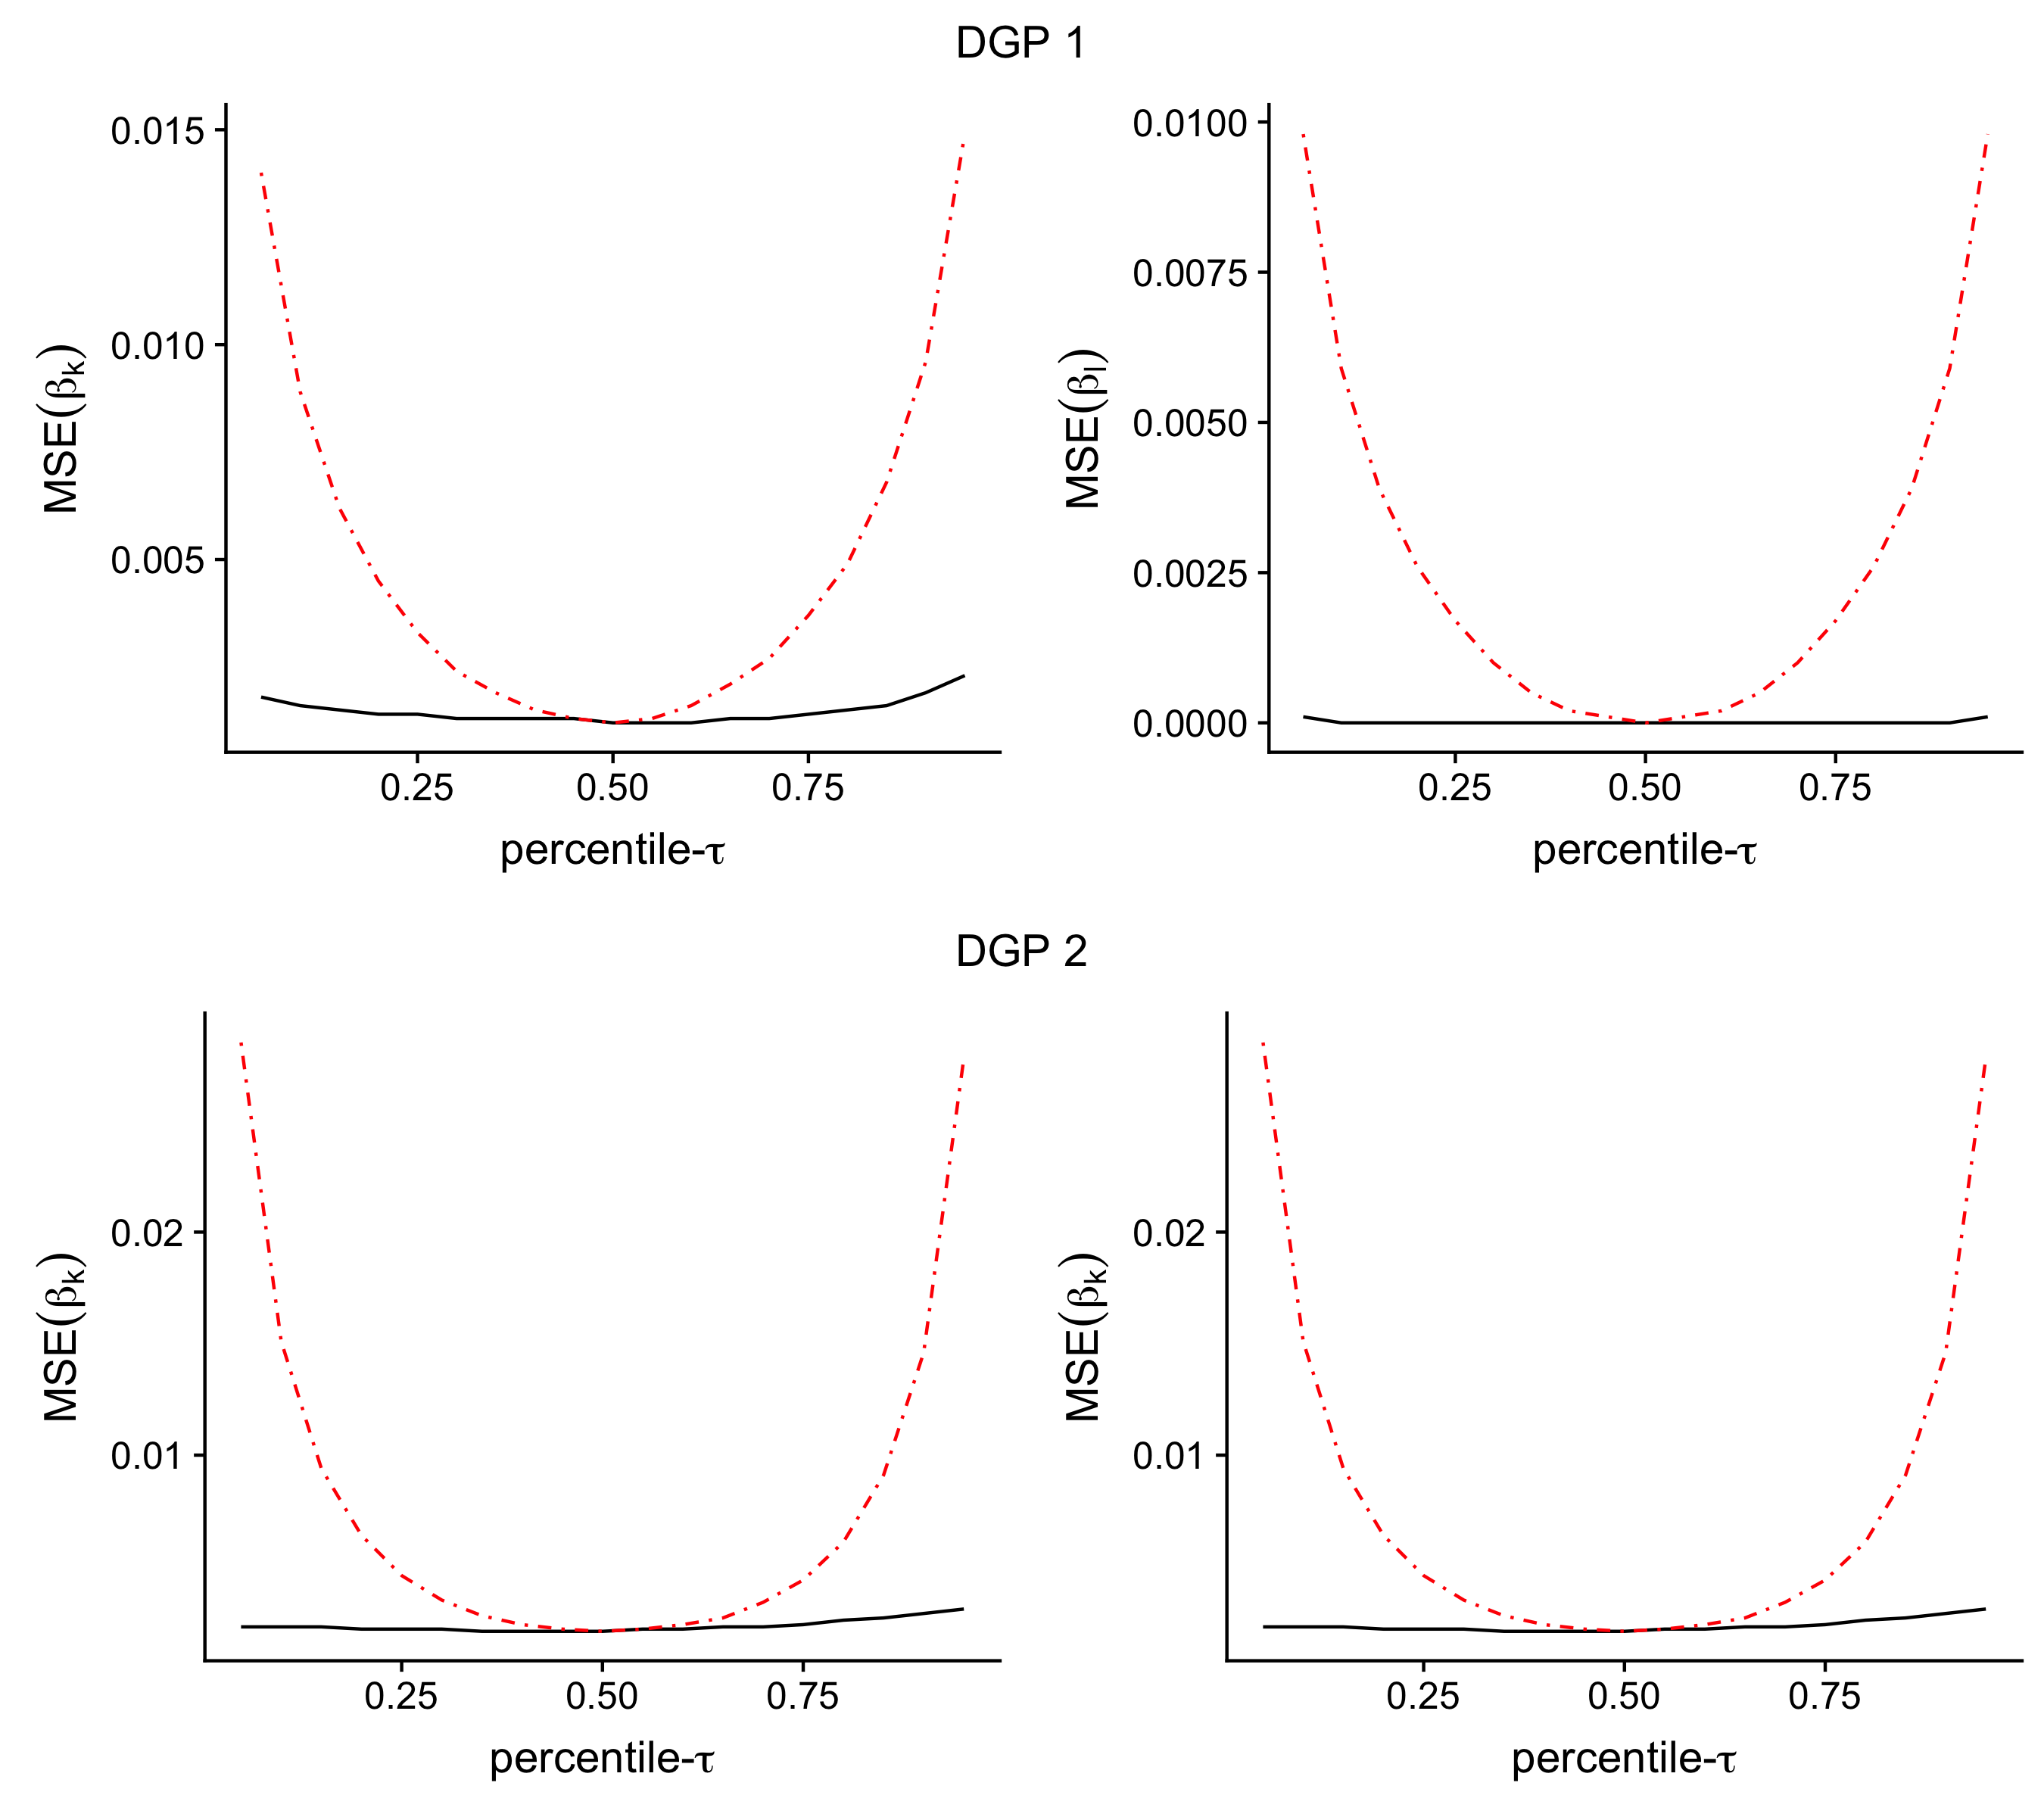
\includegraphics[width=9cm, height=9cm]{/Users/justindoty/Documents/Research/Dissertation/Production_QR_Proxy/Code/Monte_Carlo/MSE_Plot.png}
\label{fig:MSE}
\end{figure}

\begin{figure}[ht]
\centering
\caption{Difference between QLP estimators and QR estimates of $\beta_{k}(\tau)$ and $\beta_{l}(\tau)$s.}
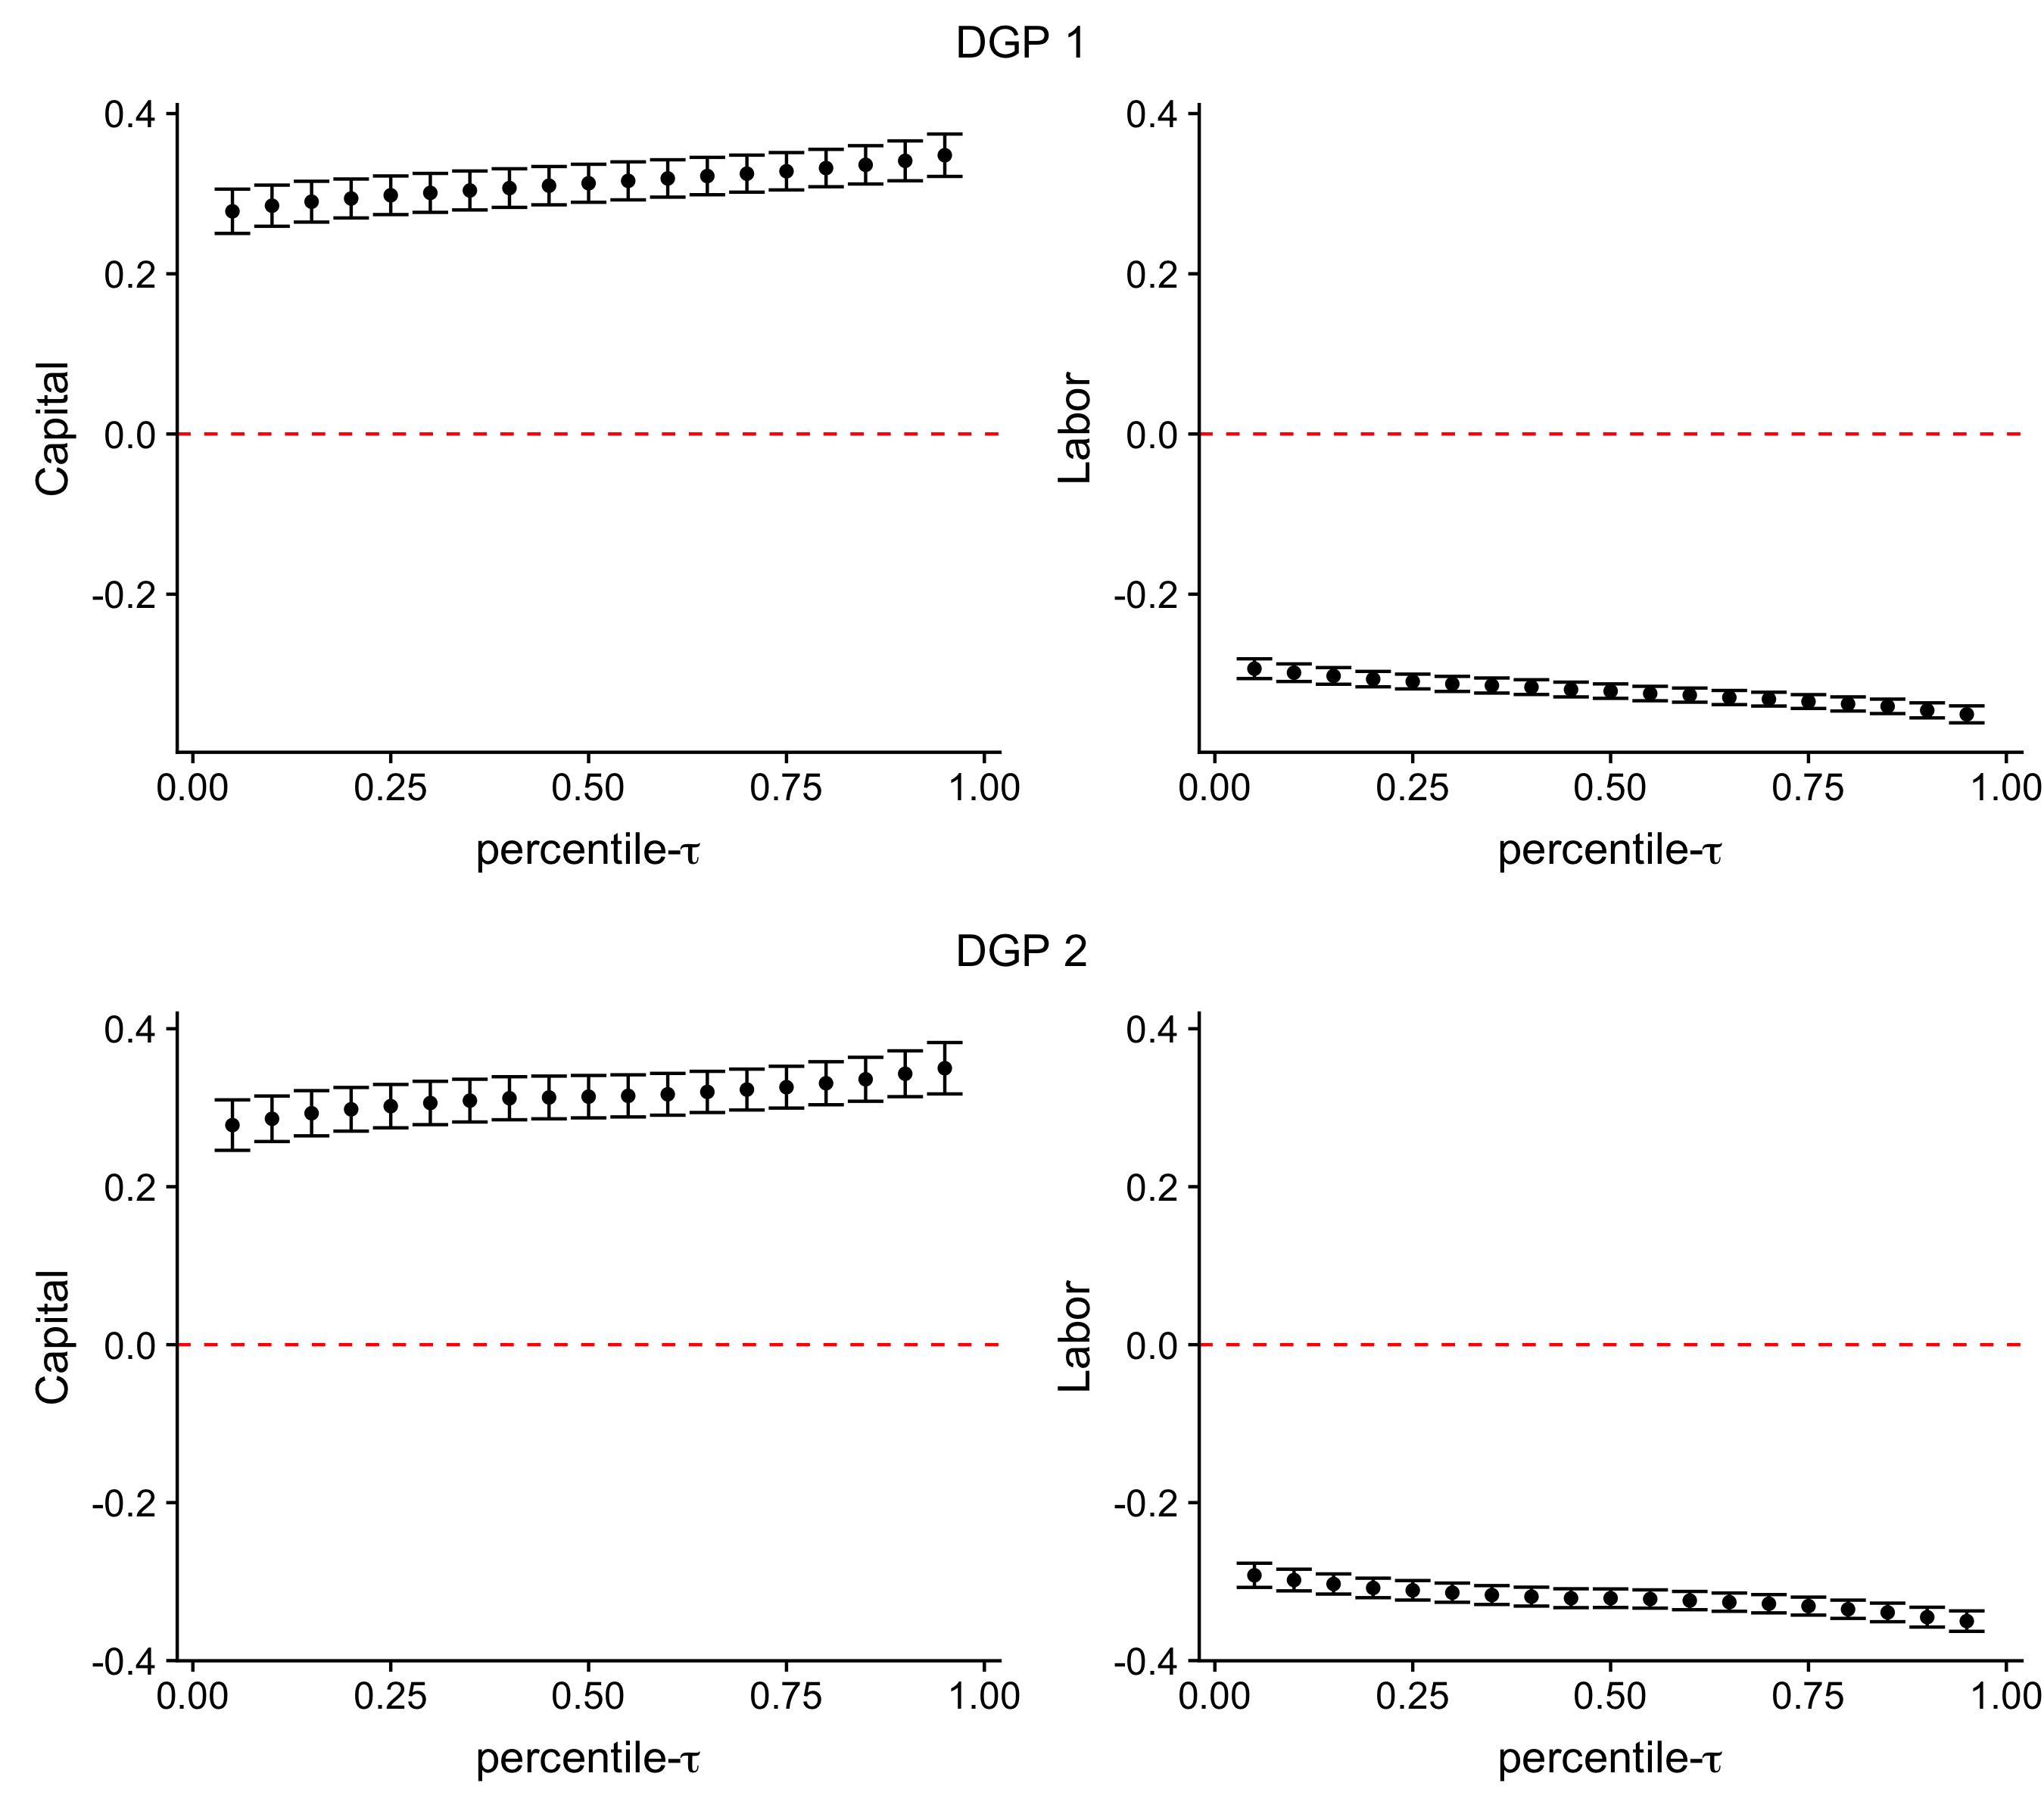
\includegraphics[width=9cm, height=9cm]{/Users/justindoty/Documents/Research/Dissertation/Production_QR_Proxy/Code/Monte_Carlo/Qdif_Plot.png}
\label{fig:QDIF}
\end{figure}

\newpage
\section{Application} \label{application}
We apply our estimator to popular firm and plant level manufacturing datasets from the US, Chile, and Colombia to examine heterogeneity in the output distribution \footnote{We thank Mert Demirer for providing the datasets from Chile and Colombia}. For each country we examine estimates across different manufacturing industries as well as how these estimates have changed over time. We use the QLP estimator presented in this paper and compare it to the LP estimates. We also compare our estimates to the quantile regression estimates without controlling for productivity. In the LP estimation procedure, we estimate the labor coefficient and $\Phi$ with a 3rd degree polynomial with interactions in capital and materials. To estimate capital, we use the LP criterion function mentioned earlier. Since we only need a consistent estimator of the production function parameters, we do not consider any over-identification conditions in this step. We use bootstrap to estimate standard errors of $\beta_{k}(\tau)$ and $\beta_{l}(\tau)$ with the number of iterations set to $500$.
\subsection{US Compustat}
The source for the US manufacturing data is from Compustat which covers publicly traded firms and contains data from their financial statements. We collect a sample between 1961 and 2010 on sales, capital expenditures, number of workers, and other expenses to construct measures of output, capital, labor, and material inputs using 3-digit deflators from \cite{nber}. Data preparation follows \cite{Keller2009} and \cite{mert}. Some issues regarding the Compustat dataset is that since the data is reported in the firm's financial statements, deflated output and input measures may not completely capture firm's actual usage. Also, since this sample only contains publicly traded firms, it is only a fraction of all manufacturing firms in the US. Summary statistics for these deflated values are provided in Table 1. We present a series of output elasticity estimates in Table 2 which are illustrated graphically in Figures \ref{fig:31coef}, \ref{fig:32coef}, \ref{fig:33coef}, and \ref{fig:USallcoef}.

Estimates of the capital elasticity are slightly increasing in the firm-size distribution in every industry as well as the combined sample. The estimates for labor elasticity for each industry and the combined sample are decreasing. For NAICS 33, the labor elasticity increases at very small $\tau$, but then decreases. In each industry, there is evidence that our model captures some heterogeneity compared to the LP model. In NAICS 31, the capital elasticity is smaller and the labor elasticity is larger than the LP estimates for very small $\tau$. In NAICS 32, there is more heterogeneity in the tails of the firm-size distribution than NAICS 32 for capital estimates, but only the labor estimates are lower than the LP estimate for very large $\tau$. The same relationship in these estimates is true in NAICS 33 and in the combined sample.
 
% latex table generated in R 3.4.1 by xtable 1.8-2 package
% Fri Mar  5 12:36:22 2021
\begin{table}[H]
\centering
\begin{tabular}{ccccccc}
  \hline\hline Industry (NAICS code) &   & 1st Qu. & Median & 3rd Qu. & Mean & sd \\ 
  \hline
31 (Total=3271) & Output & 19.05 & 20.24 & 21.57 & 20.3 & 1.77 \\ 
   & Capital & 18.66 & 20.37 & 21.76 & 20.19 & 2.12 \\ 
   & Labor & 17.42 & 19.08 & 20.61 & 19.02 & 2.21 \\ 
   & Materials & 17.96 & 19.59 & 21.15 & 19.54 & 2.21 \\ 
  32 (Total=7207) & Output & 15.67 & 17.04 & 18.51 & 17.01 & 2.05 \\ 
   & Capital & 15.65 & 17.51 & 19.13 & 17.31 & 2.41 \\ 
   & Labor & 14.44 & 16.01 & 17.57 & 16.01 & 2.29 \\ 
   & Materials & 14.89 & 16.53 & 18.25 & 16.52 & 2.37 \\ 
  33 (Total=13978) & Output & 7.38 & 8.58 & 9.8 & 8.5 & 1.67 \\ 
   & Capital & 6.67 & 8.29 & 9.74 & 8.15 & 1.95 \\ 
   & Labor & 6.01 & 7.42 & 8.91 & 7.48 & 1.93 \\ 
   & Materials & 6.33 & 7.82 & 9.29 & 7.82 & 1.95 \\ 
  All (Total=24456) & Output & 18.58 & 19.78 & 21.23 & 19.85 & 1.79 \\ 
   & Capital & 18.14 & 19.86 & 21.26 & 19.67 & 2.16 \\ 
   & Labor & 16.98 & 18.59 & 20.13 & 18.56 & 2.17 \\ 
   & Materials & 17.49 & 19.12 & 20.66 & 19.06 & 2.2 \\ 
   \hline
\end{tabular}
\end{table}

\label{Tab:USsummary}


\begin{figure}[H]
\centering
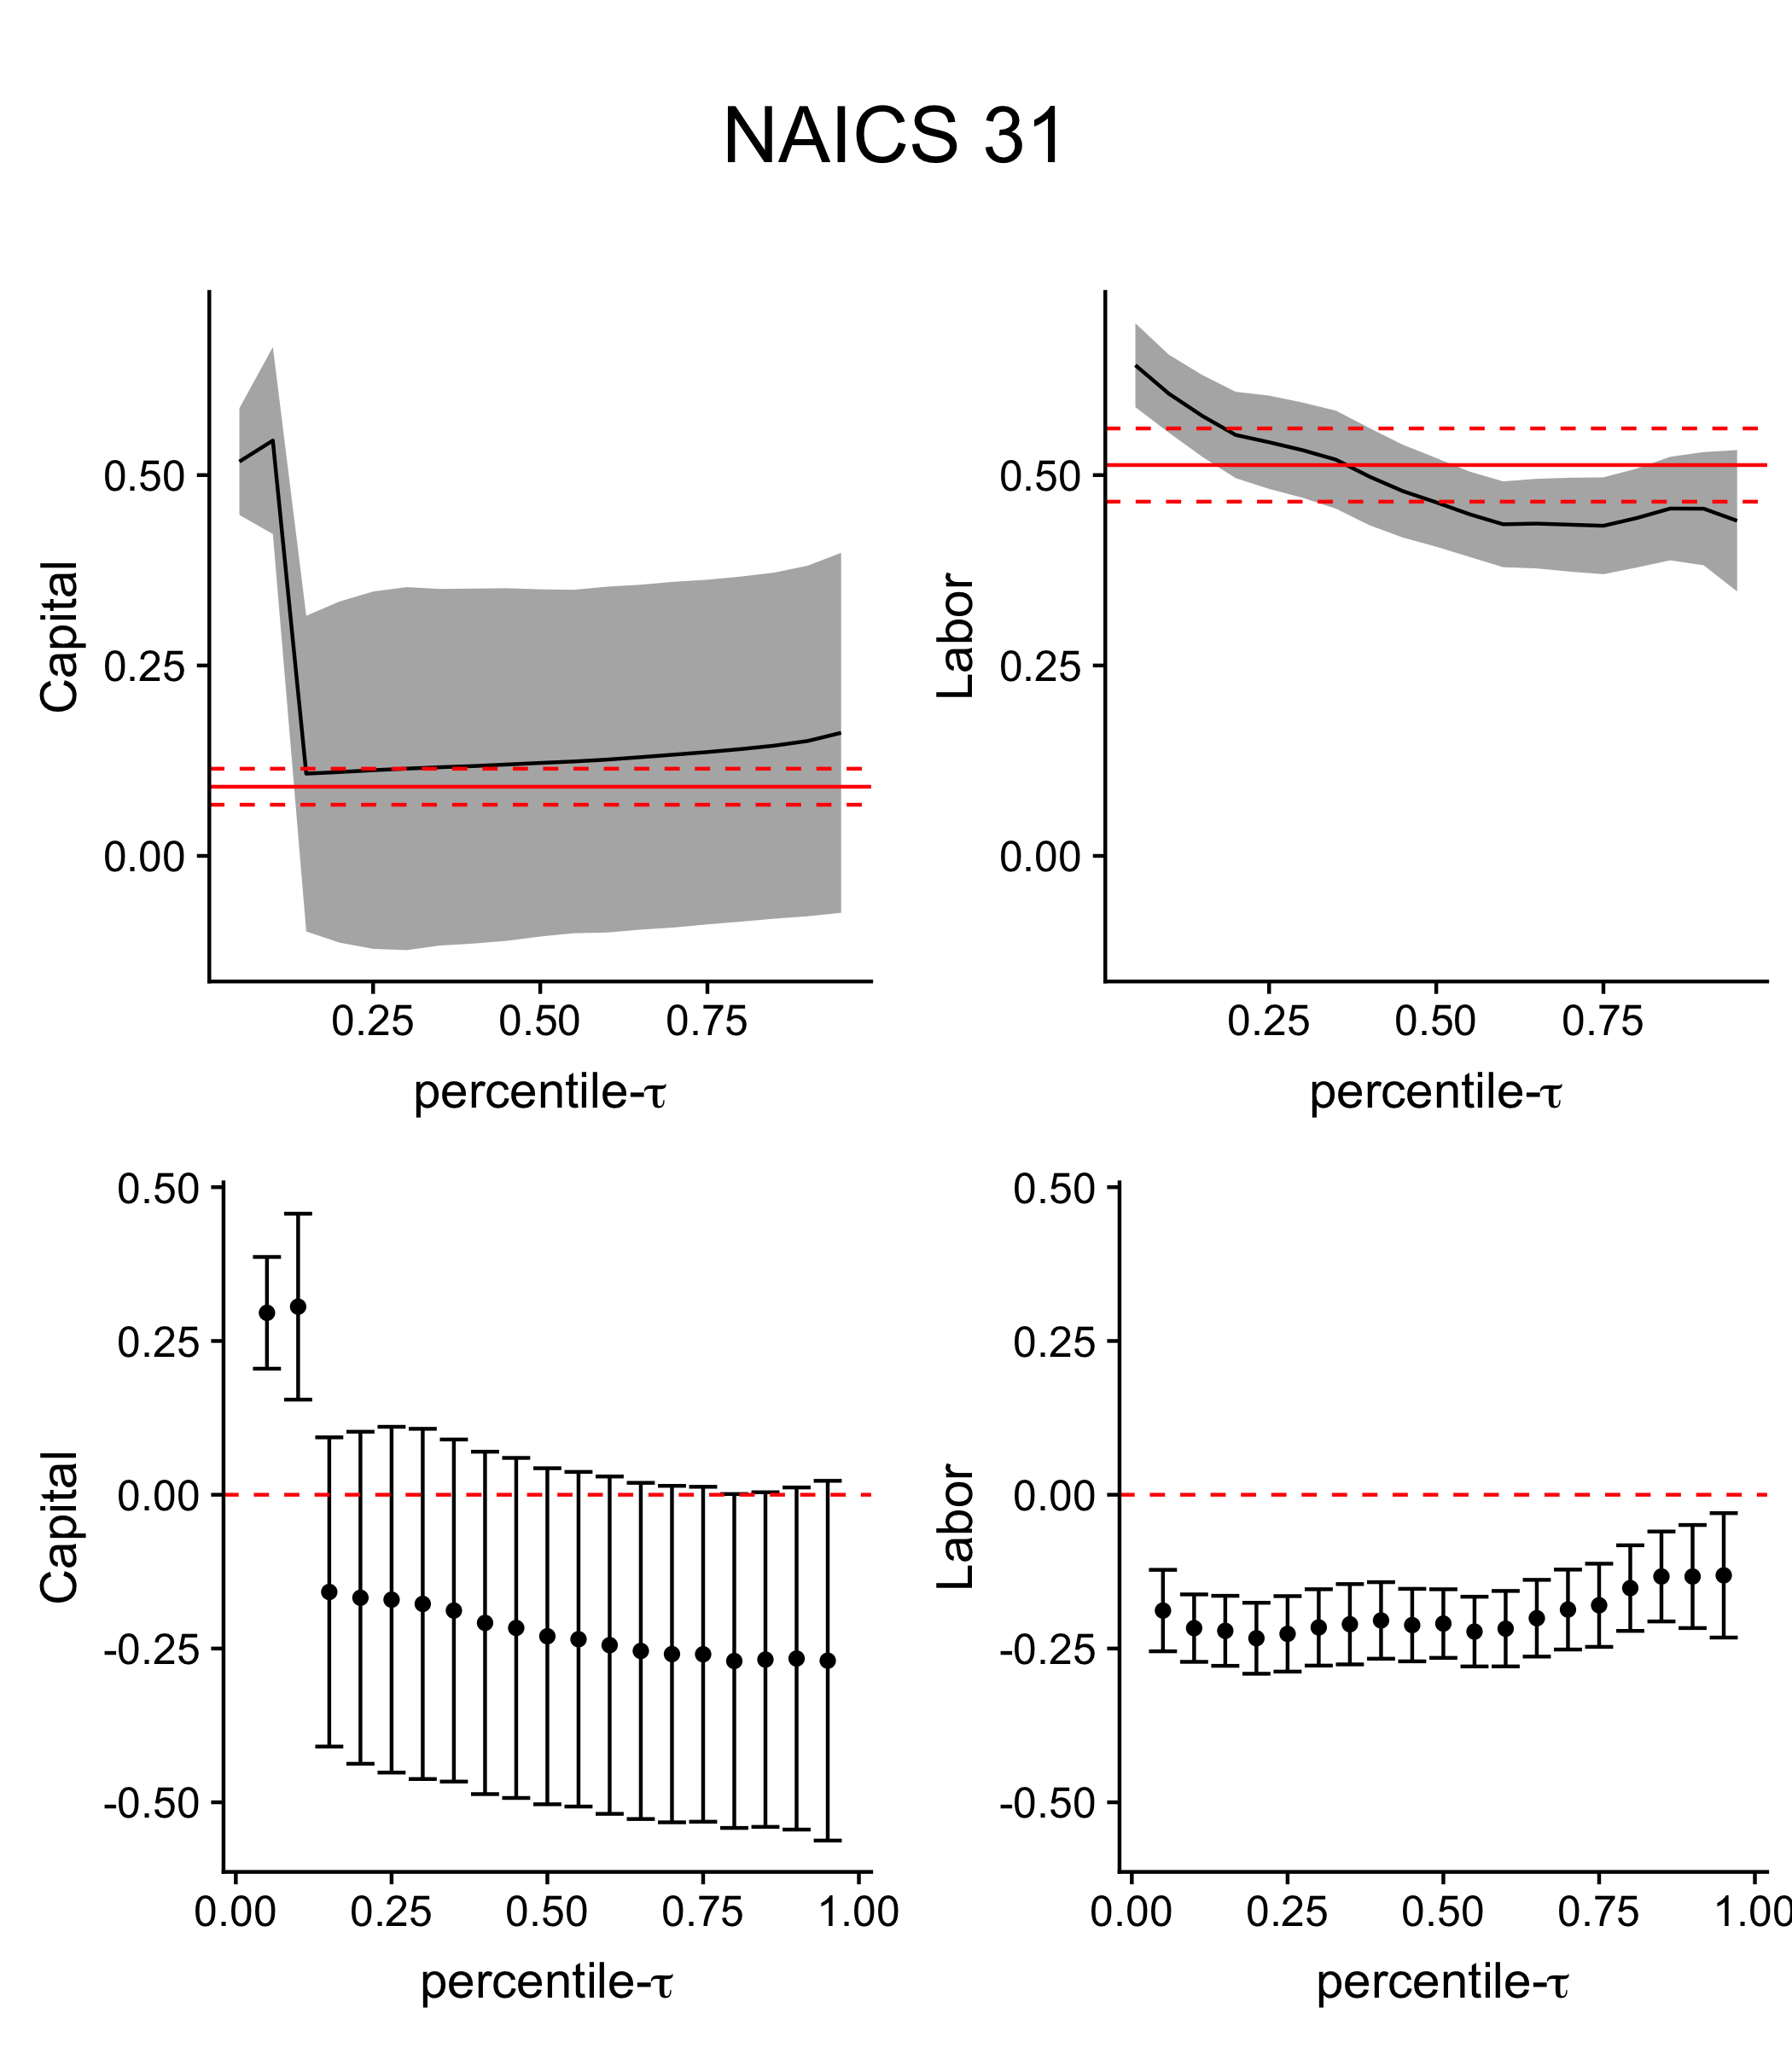
\includegraphics[width=9cm, height=9cm]{/Users/justindoty/Documents/Research/Dissertation/Production_QR_Proxy/Code/Empirical/US/Plots/Coef_Plot_NAICS_31.png}
\caption{Top row: Estimated values of production function coefficients and their point-wise 90\% confidence interval. Bottom row: Difference between QLP and quantile regression estimates and their 95\% confidence intervals.}
\label{fig:31coef}
\end{figure}

\begin{figure}[H]
\centering
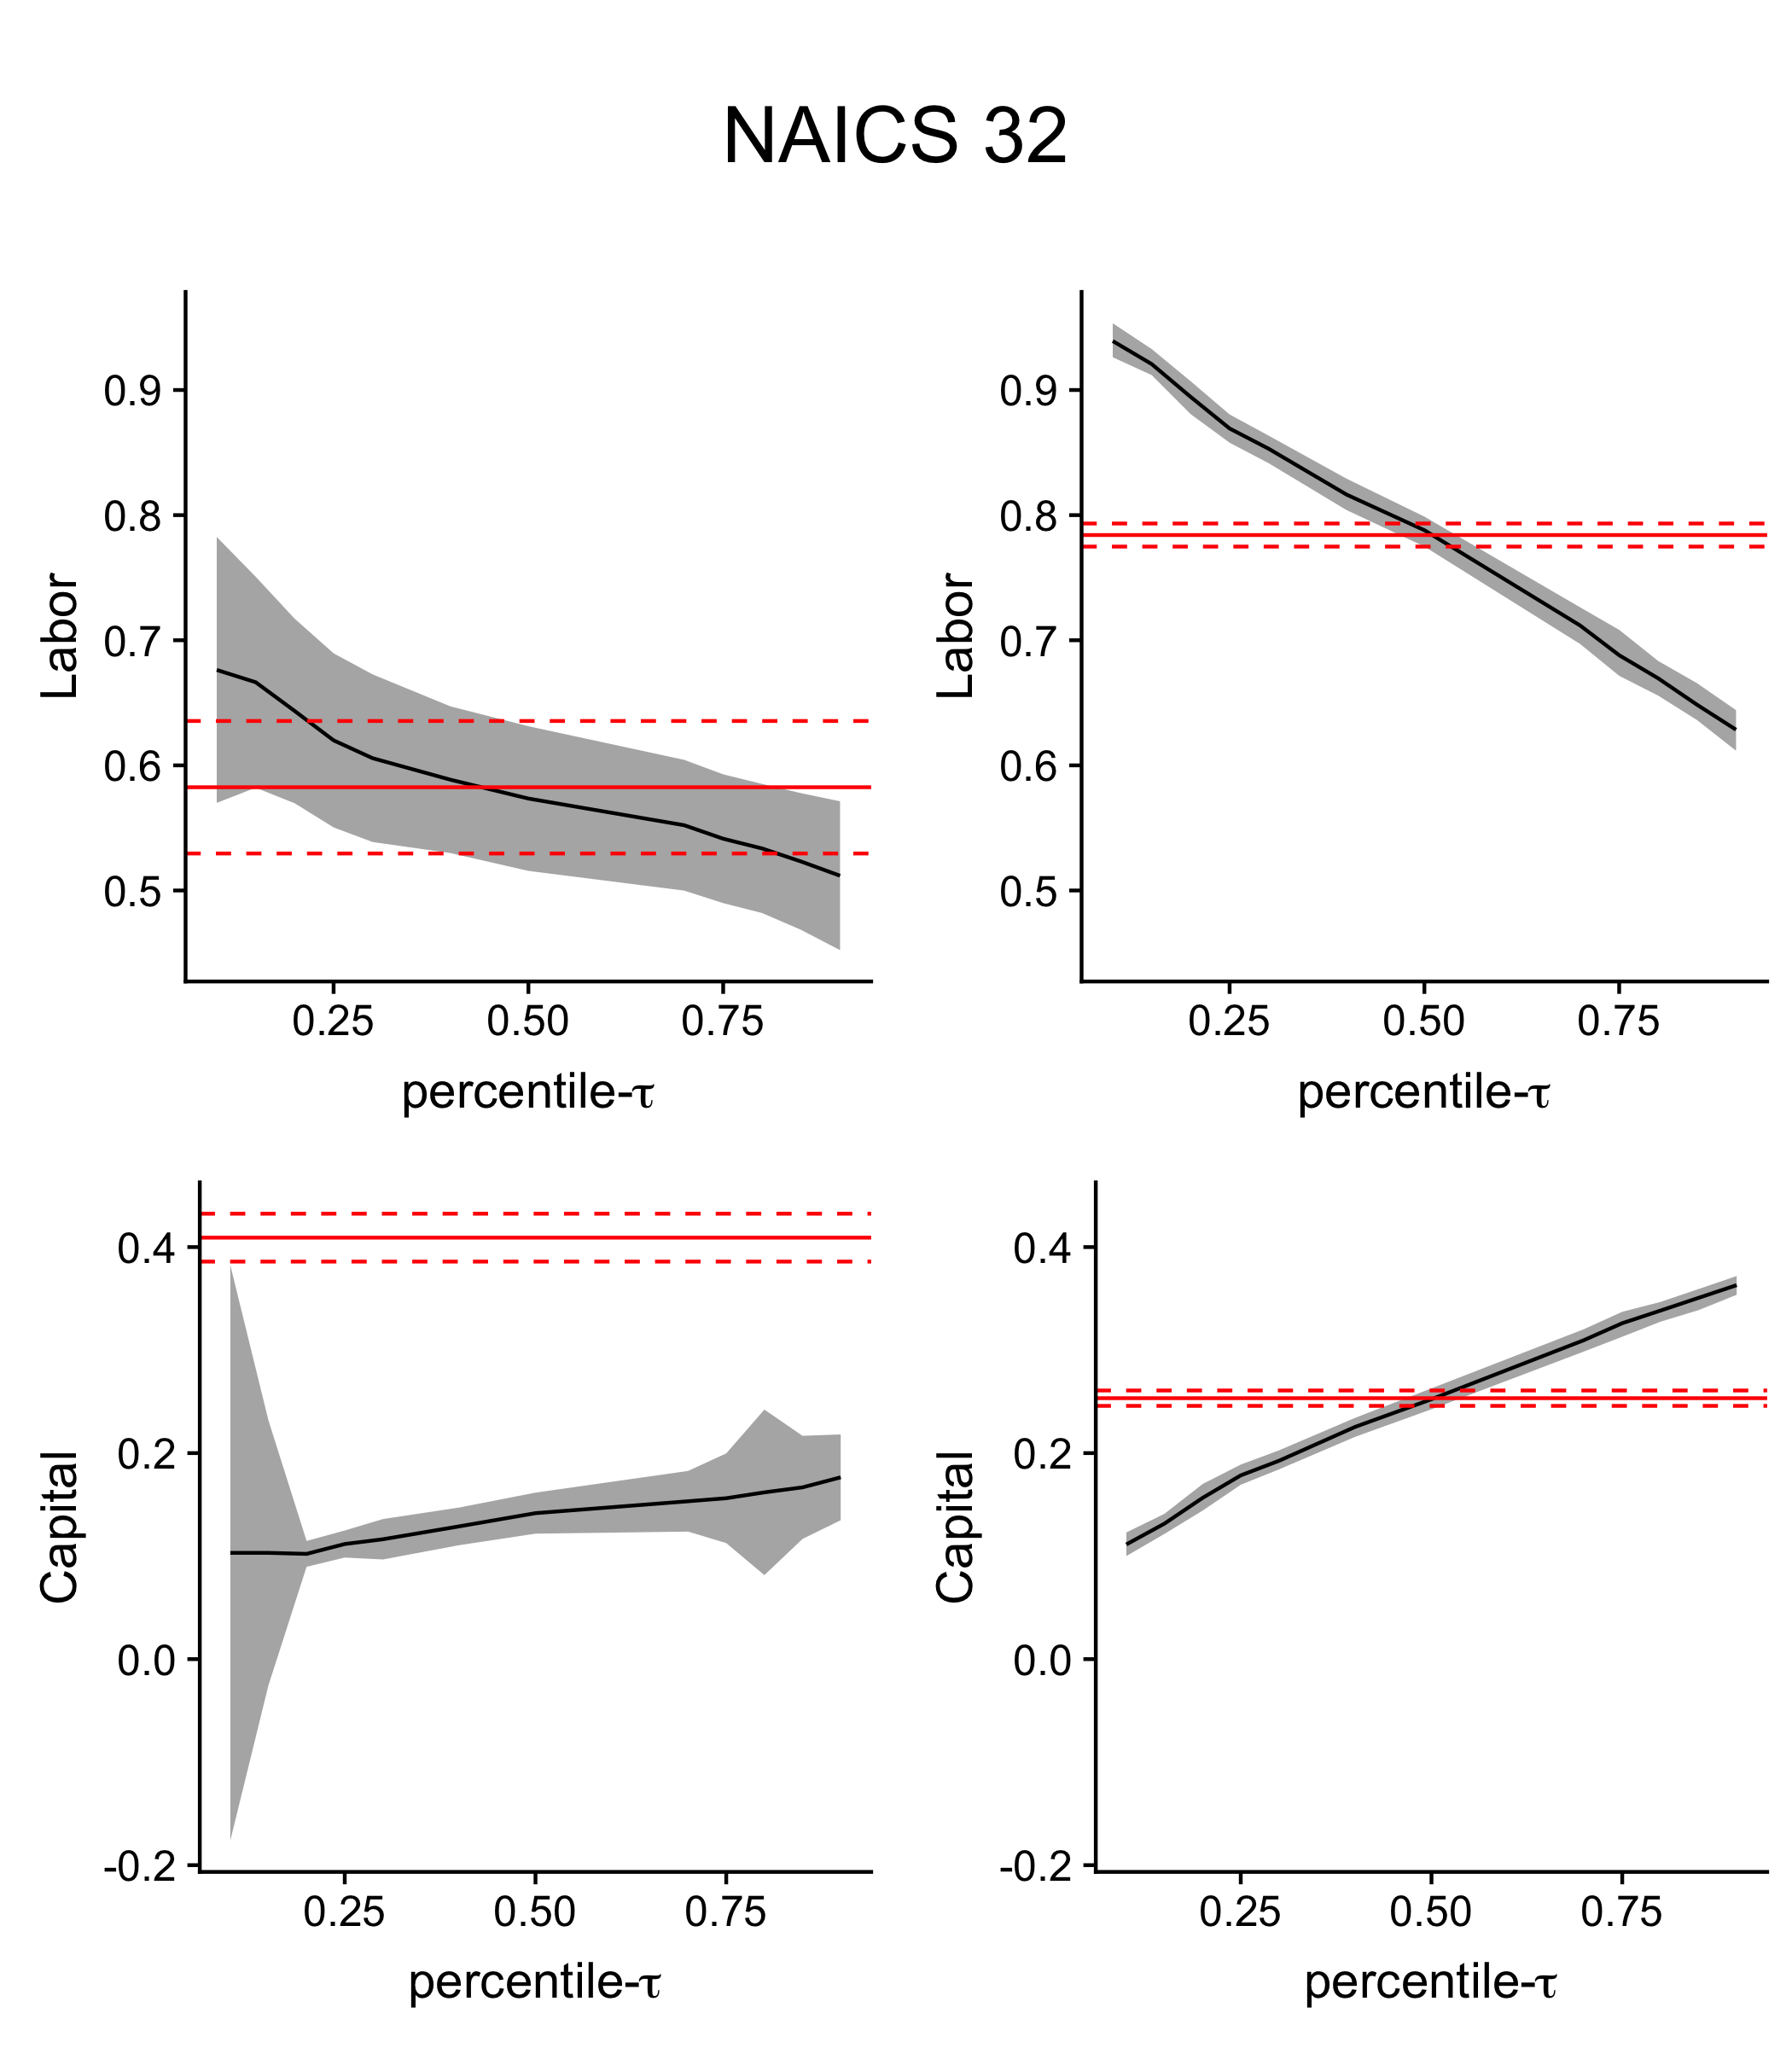
\includegraphics[width=9cm, height=9cm]{/Users/justindoty/Documents/Research/Dissertation/Production_QR_Proxy/Code/Empirical/US/Plots/Coef_Plot_NAICS_32.png}
\caption{Top row: Estimated values of production function coefficients and their point-wise 90\% confidence interval. Bottom row: Difference between QLP and quantile regression estimates and their 95\% confidence intervals.}
\label{fig:32coef}
\end{figure}

\begin{figure}[H]
\centering
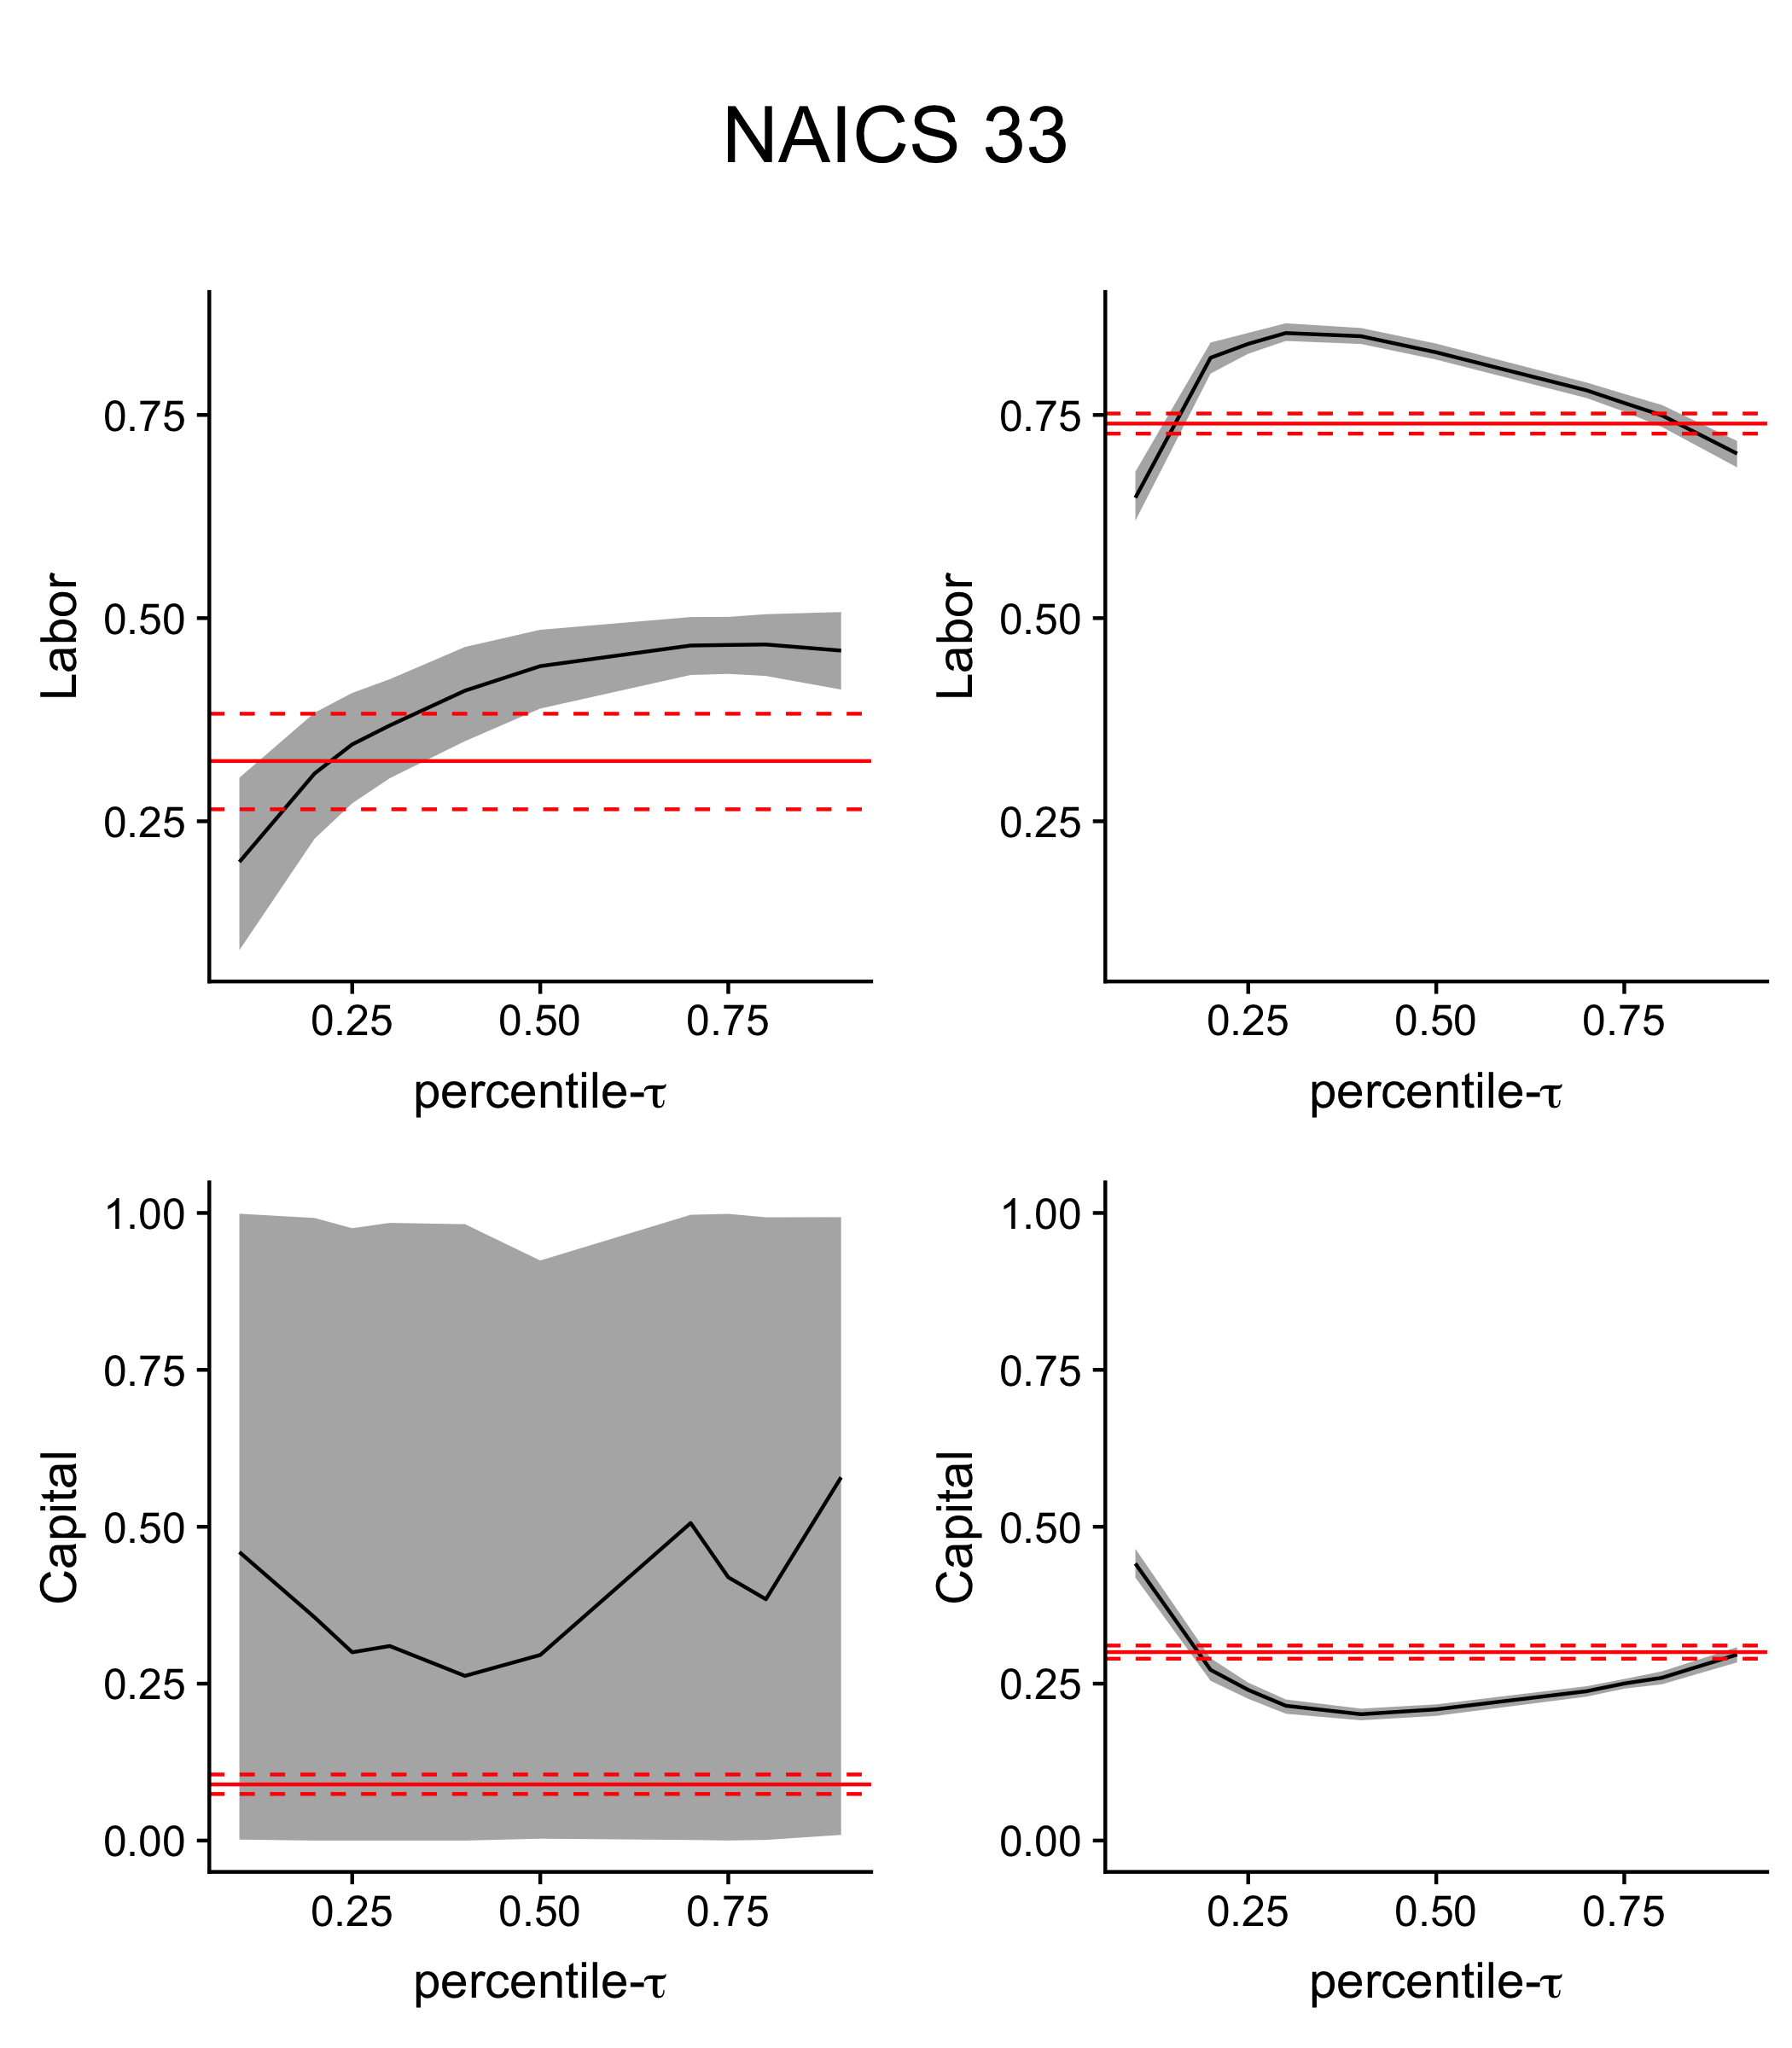
\includegraphics[width=9cm, height=9cm]{/Users/justindoty/Documents/Research/Dissertation/Production_QR_Proxy/Code/Empirical/US/Plots/Coef_Plot_NAICS_33.png}
\caption{Top row: Estimated values of production function coefficients and their point-wise 90\% confidence interval. Bottom row: Difference between QLP and quantile regression estimates and their 95\% confidence intervals.}
\label{fig:33coef}
\end{figure}

\begin{figure}[H]
\centering
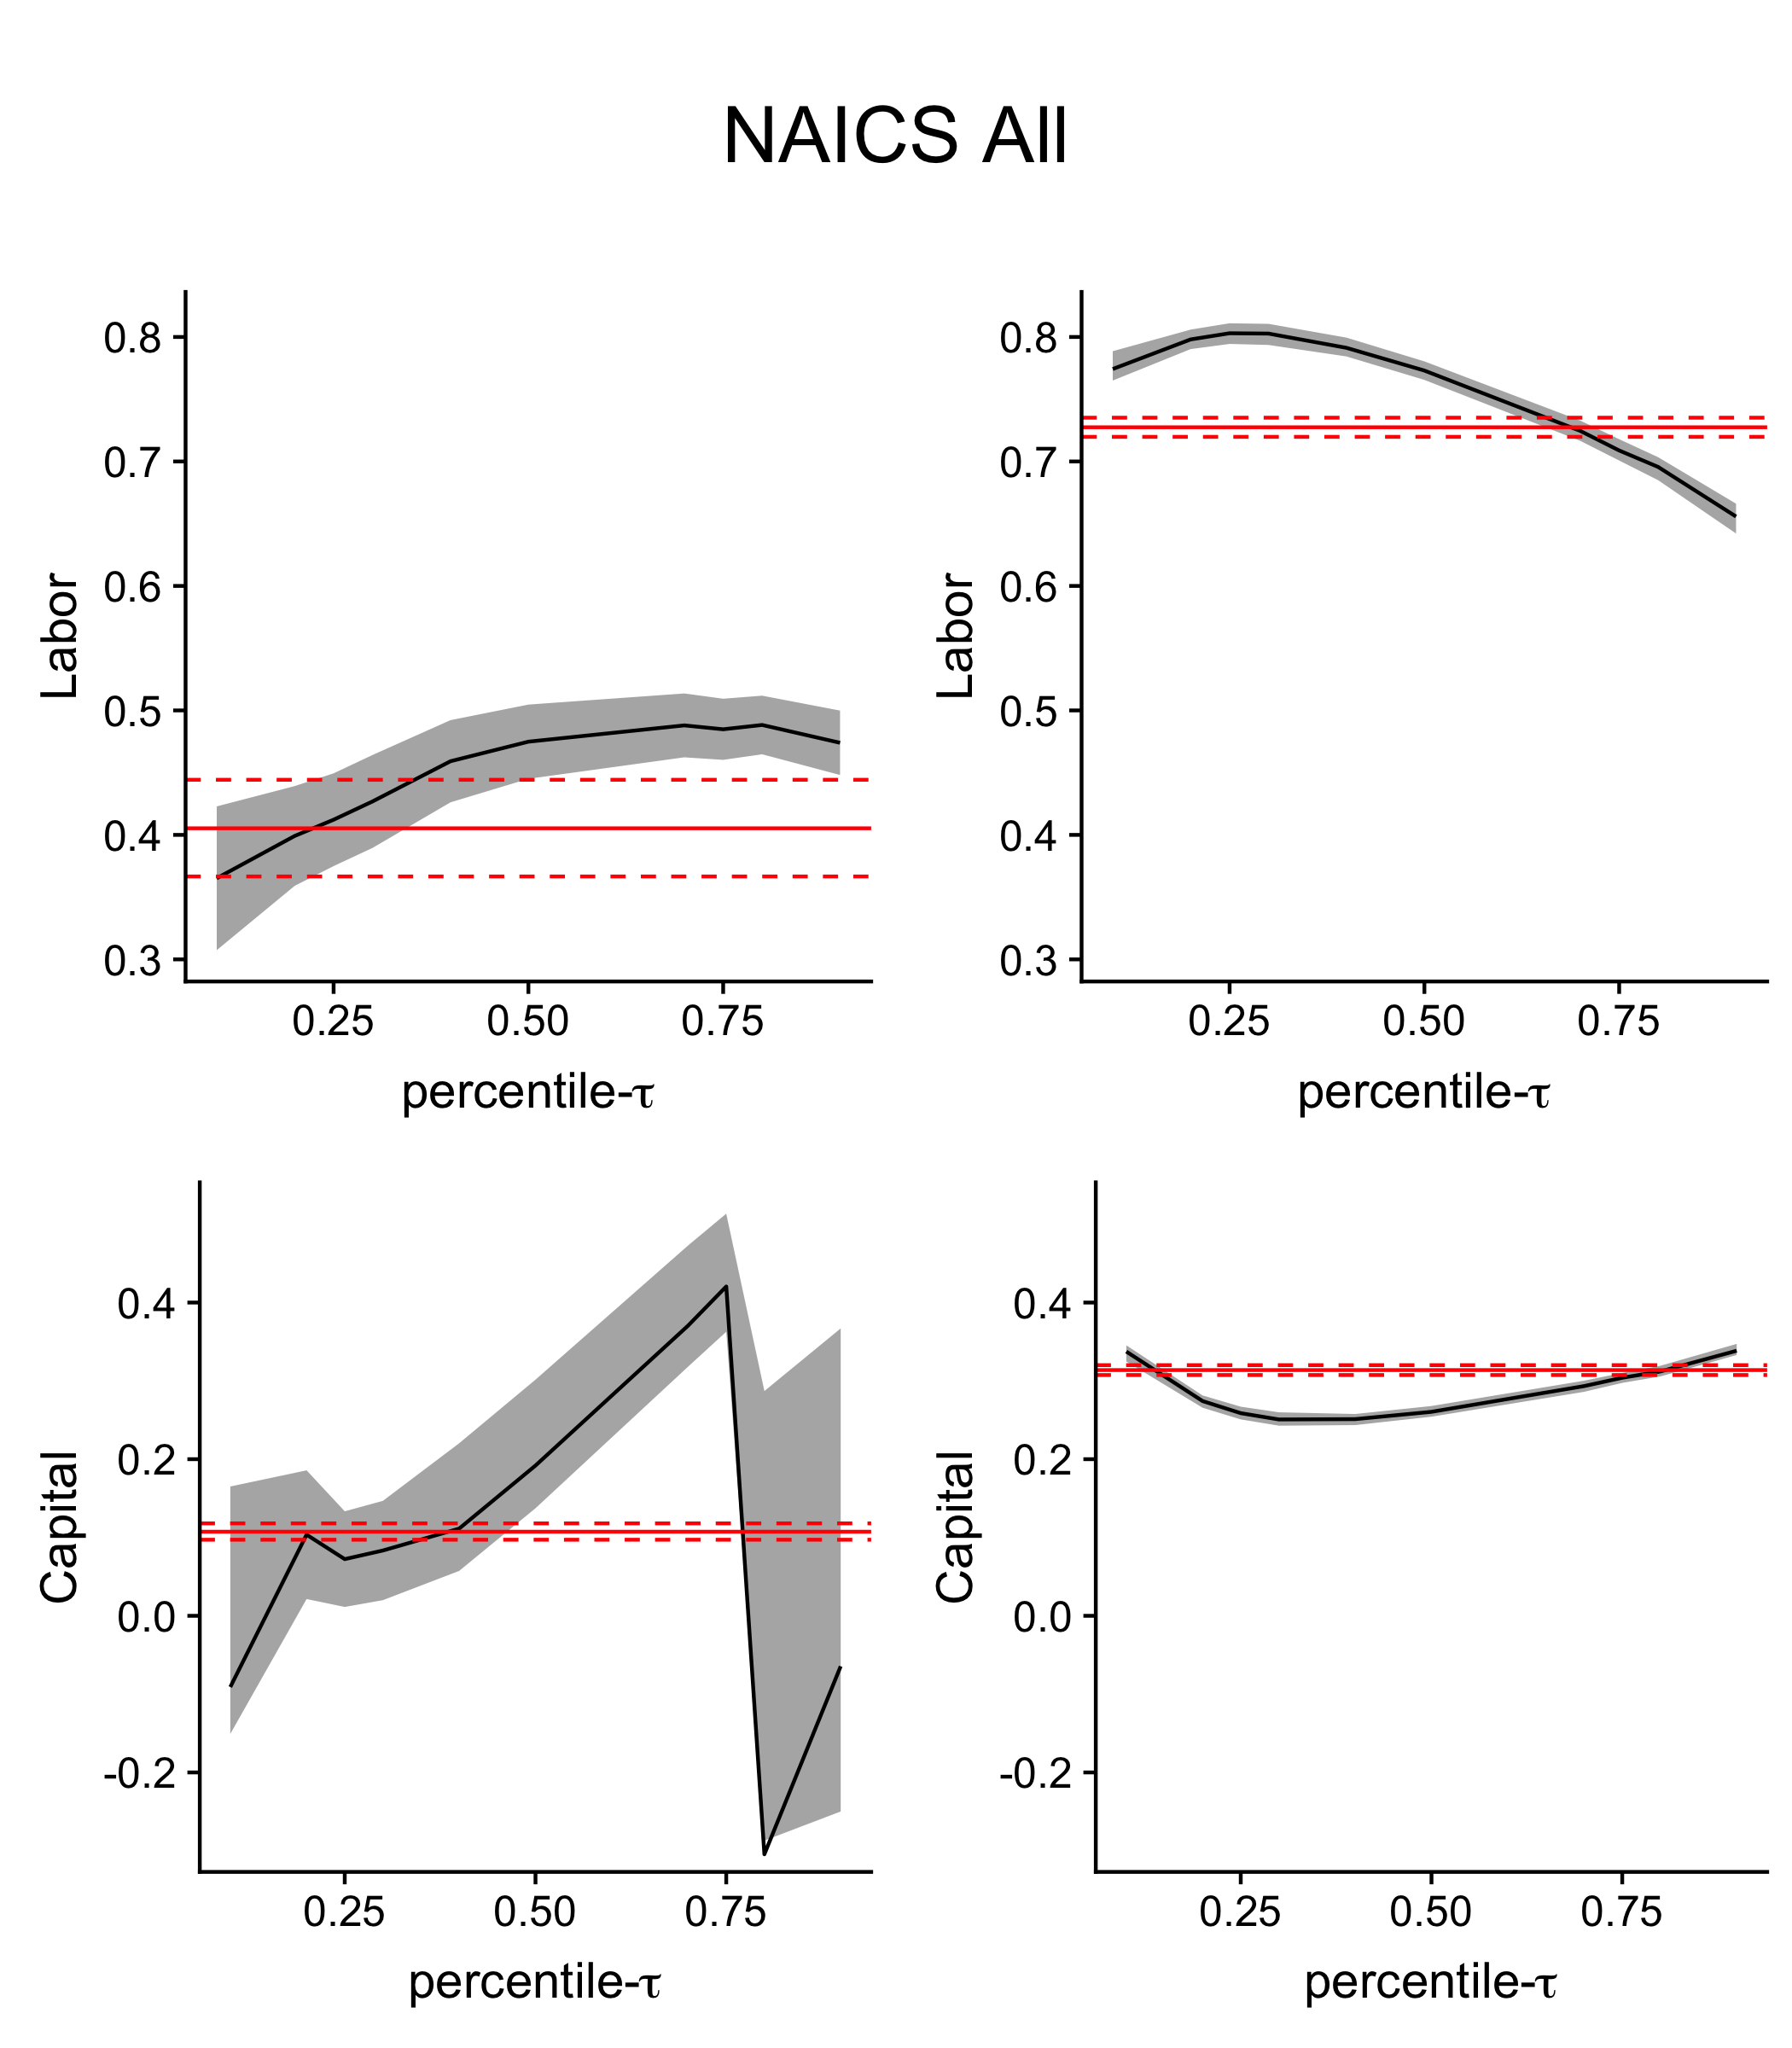
\includegraphics[width=10cm, height=11cm]{/Users/justindoty/Documents/Research/Dissertation/Production_QR_Proxy/Code/Empirical/US/Plots/Coef_Plot_NAICS_All.png}
\caption{Top row: Estimated values of production function coefficients and their point-wise 90\% confidence interval. Bottom row: Difference between QLP and quantile regression estimates and their 95\% confidence intervals.}
\label{fig:USallcoef}
\end{figure}

In each industry we compare the difference between QLP and QR estimates to test whether our model corrects for endogeneity from unobserved productivity. Bootstrap is used to construct confidence intervals of the difference between the two estimates. We find that there are significant differences between these estimates in all of the samples. This suggests that even after controlling for productivity differences across firms, there is still unexplained heterogeneity between firms.

We use the estimates from the output elasticities to construct measures of returns to scale and capital intensity in Table 3. The results for returns to scale are puzzling as they are all significantly different from constant returns to scale. Each sample and each quantile of firm-size exhibits large decreasing returns to scale and these returns decrease when $\tau$ increases. Previous papers that estimate returns to scale using the Compustat dataset such as \cite{Keller2009} and \cite{mert} show constant returns to scale using a gross-output production function. Therefore it is possible that the empirical value-added (deflated sales minus intermediate input expenditure) is a poor proxy for value-added in our model and that value-added biases the returns to scale estimates. Differences in returns to scale in value-added and gross-output production functions are explored by \cite{Basu1997}. We also report estimates of capital intensity measured by the ratio of capital to labor elasticity for each quantile. Each industry has estimates of capital intensity that increases with $\tau$. This result is consistent with previous findings such as \cite{Holmes2008}, \cite{Kumar1999} and \cite{mert}.


% latex table generated in R 3.4.1 by xtable 1.8-2 package
% Wed Feb  3 20:38:50 2021
\begin{table}[ht]
\centering
\caption{Coefficient Estimates and Standard Errors for US Manufacturing Firms} 
\begin{tabular}{cccccccccc}
  \hline\hline & & \multicolumn{2}{c}{Capital}  & \multicolumn{2}{c}{Labor} & \multicolumn{2}{c}{Returns to Scale} & \multicolumn{2}{c}{Capital Intensity}\\ \cmidrule(lr){3-4} \cmidrule(lr){5-6} \cmidrule(lr){7-8} \cmidrule(lr){9-10}NAICS & $\tau$ & Coef. & s.e & Coef. & s.e & Coef. & s.e & Coef. & s.e \\ 
  \hline
31 & 0.10 & 0.563 & 0.0764 & 0.607 & 0.0311 & 1.170 & 0.0816 & 0.928 & 0.1368 \\ 
   & 0.25 & 0.113 & 0.1476 & 0.543 & 0.0372 & 0.656 & 0.1478 & 0.208 & 0.2740 \\ 
   & 0.50 & 0.122 & 0.1388 & 0.464 & 0.0354 & 0.586 & 0.1468 & 0.263 & 0.2994 \\ 
   & 0.90 & 0.147 & 0.1359 & 0.456 & 0.0452 & 0.603 & 0.1452 & 0.322 & 0.3178 \\ 
  32 & 0.10 & 0.081 & 0.1043 & 0.654 & 0.0497 & 0.735 & 0.0816 & 0.123 & 0.1594 \\ 
   & 0.25 & 0.092 & 0.0577 & 0.605 & 0.0332 & 0.697 & 0.0615 & 0.152 & 0.0992 \\ 
   & 0.50 & 0.102 & 0.0624 & 0.561 & 0.0264 & 0.663 & 0.0666 & 0.182 & 0.1130 \\ 
   & 0.90 & 0.124 & 0.0647 & 0.526 & 0.0307 & 0.649 & 0.0725 & 0.235 & 0.1341 \\ 
  33 & 0.10 & 0.014 & 0.0488 & 0.210 & 0.0598 & 0.223 & 0.0728 & 0.066 & 0.3861 \\ 
   & 0.25 & 0.043 & 0.0499 & 0.354 & 0.0432 & 0.397 & 0.0618 & 0.121 & 0.1664 \\ 
   & 0.50 & 0.064 & 0.0478 & 0.439 & 0.0304 & 0.503 & 0.0541 & 0.146 & 0.1164 \\ 
   & 0.90 & 0.098 & 0.0476 & 0.446 & 0.0287 & 0.544 & 0.0524 & 0.220 & 0.1133 \\ 
  All & 0.10 & 0.049 & 0.0410 & 0.363 & 0.0420 & 0.412 & 0.0547 & 0.135 & 0.1558 \\ 
   & 0.25 & 0.070 & 0.0373 & 0.411 & 0.0257 & 0.481 & 0.0437 & 0.169 & 0.1017 \\ 
   & 0.50 & 0.087 & 0.0322 & 0.470 & 0.0201 & 0.558 & 0.0365 & 0.186 & 0.0754 \\ 
   & 0.90 & 0.117 & 0.0322 & 0.474 & 0.0179 & 0.591 & 0.0352 & 0.247 & 0.0748 \\ 
   \hline
\end{tabular}
\end{table}


We also use our quantile production function estimates to construct measures of firm level productivity which we define as
\begin{equation}
\hat{w}_{it,\tau}=\exp(y_{it}-\hat{\beta_{k}}(\tau)k_{it}-\hat{\beta_{l}}(\tau)l_{it})
\end{equation}
We use these measures to compare productivity growth over time to LP estimates over the distribution of firm-size. Figure \ref{fig:USpgrowth} reports average productivity for all US firms in the sample with the base year of the sample period set to 100. We can see that productivity growth was rapid in the beginning of the sample period but then declined after 1970 and increase again after 1980. Growth trends for each percentile of firm-size were similar although larger firms in this sample were more productive than smaller ones. The LP estimates are close to the productivity estimates for medium-sized firms at $\tau=0.5$.

We are also interested in examining the firm-size distribution over time and whether there are differences in within-firm and across firm technology heterogeneity. Figure \ref{fig:UStimecoef} plots estimates of the output elasticities over 5 year intervals. For labor elasticity, there is heterogeneity across the firm-size distribution in the beginning of the sample period. Larger firms had greater estimates of labor elasticity than small firms. This heterogeneity decreases up until 1980 when the relationship between firm-size and labor elasticity reverses. At the end of our sample period, very large firms have smaller estimates of labor elasticity than very small firms. Large firms have higher estimates of capital elasticity than small and medium-sized firms. These estimates are increasing until the year 2000 then decrease with the relationship between firm-size and capital estimates holding throughout this period.


\begin{figure}[H]
\centering
\includegraphics[width=10cm]{/Users/justindoty/Documents/Research/Dissertation/Production_QR_Proxy/Code/Empirical/US/Plots/TFP_Plot.png}
\caption{Estimated average productivity over time for the US. Base productivity in 1961 is set to 100.}
\label{fig:USpgrowth}
\end{figure}

\begin{figure}[H]
\centering
\includegraphics[width=10cm]{/Users/justindoty/Documents/Research/Dissertation/Production_QR_Proxy/Code/Empirical/US/Plots/Time_Plot.png}
\caption{Estimated values of production function coefficients over time estimated at 5 year intervals}
\label{fig:UStimecoef}
\end{figure}


%----------------------------------------------------------------------------------------

\subsection{Chilean Manufacturing}
This data comes from the census of Chilean manufacturing plants conducted by the Instituto Nacional de Estadist\'ica (INE). The sample is collected between 1979 and 1996 for firms with more than 10 employees. We divide our estimates into the three largest manufacturing industries: Food (ISIC 311), Fabricated Metals (ISIC 381), and Textiles (ISIC 321). We also aggregate the three industries with the other smaller industries to obtain estimates from the entire sample. Summary statistics for the data we use are provided in Table 4.

Figures \ref{fig:CHL311}, \ref{fig:CHL321}, and \ref{fig:CHL381} illustrate our estimates from our model compared to LP estimates as well as their differences to QR estimates. In each industry and the combined sample, estimates of capital elasticity are increasing in firm-size. In ISIC 311 and ISIC 381, the our model estimates lower capital elasticities than LP estimates for small $\tau$. In ISIC 321 and the combined sample, there are differences between these estimates for both small and large $\tau$. The labor estimates in ISIC 311 are increasing and different than the LP estimate for large $\tau$. In ISIC 321, labor estimates are decreasing and not different from the LP estimate. In ISIC 381, labor estimates are mostly constant and not different from the LP estimate. Finally, in the combined sample, our estimates exhibit a U-shaped relationship although overall these are not different from the LP estimate. In ISIC 321 our capital estimates do not differ much from QR estimates. From Table 5, our estimates of returns to scale are more reasonable compared to the US estimates except for small firms who experience decreasing returns to scale. In each industry, returns to scale are increasing with firm-size. Capital intensity is increasing as well except for large firms at $\tau=0.9$ in ISIC 311.

Figure \ref{fig:CHLpgrowth} reports average productivity for all Chilean plants in the sample with base period set to 100. Productivity decreases in the beginning of the 1980s but then increases for the rest of the sample period. These estimates suggest that small firms had higher productivity than large firms. The LP estimates are similar to productivity of medium-sized firms at $\tau=0.5$. Figure \ref{fig:CHLtimecoef} shows the time trends in output elasticities. The estimate of labor elasticity are high for each quantile of firm-size and decreases steadily with the exception of small firms ($\tau=0.1$). The estimates for capital elasticities follow similar trends for each quantile. Capital elasticity estimates are higher for large firms than small firms.


% latex table generated in R 3.4.1 by xtable 1.8-2 package
% Wed Jan  6 11:45:58 2021
\begin{table}[H]
\centering
\caption{Summary Statistics (in logs) for Chile Manufacturing Data} 
\begin{tabular}{ccccccc}
  \hline\hline Industry (ISIC code) &   & 1st Qu. & Median & 3rd Qu. & Mean & sd \\ 
  \hline
311 (Total=13838) & Output & 10.21 & 10.84 & 12.22 & 11.36 & 1.58 \\ 
   & Capital & 10.56 & 11.4 & 12.4 & 11.52 & 1.37 \\ 
   & Labor & 10.49 & 11.4 & 12.54 & 11.53 & 1.43 \\ 
   & Materials & 10.38 & 11.28 & 12.53 & 11.56 & 1.6 \\ 
  381 (Total=4311) & Output & 6.69 & 7.66 & 9.06 & 8.02 & 1.98 \\ 
   & Capital & 7.52 & 8.51 & 9.7 & 8.65 & 1.68 \\ 
   & Labor & 7.21 & 8.34 & 9.56 & 8.4 & 1.72 \\ 
   & Materials & 7.22 & 8.35 & 9.72 & 8.54 & 1.92 \\ 
  321 (Total=4302) & Output & 2.77 & 3.22 & 3.91 & 3.49 & 0.99 \\ 
   & Capital & 2.89 & 3.47 & 4.22 & 3.71 & 1.08 \\ 
   & Labor & 2.94 & 3.48 & 4.37 & 3.69 & 0.95 \\ 
   & Materials & 2.89 & 3.43 & 4.28 & 3.67 & 1.02 \\ 
  All (Total=51567) & Output & 9.84 & 10.46 & 11.81 & 10.94 & 1.56 \\ 
   & Capital & 9.91 & 10.75 & 11.79 & 10.86 & 1.41 \\ 
   & Labor & 9.68 & 10.62 & 11.75 & 10.73 & 1.48 \\ 
   & Materials & 9.81 & 10.68 & 11.89 & 10.93 & 1.62 \\ 
   \hline
\end{tabular}
\end{table}
  

\begin{figure}[H]
\centering
\includegraphics[width=9cm, height=9cm]{/Users/justindoty/Documents/Research/Dissertation/Production_QR_Proxy/Code/Empirical/Chile/Plots/Coef_Plot_ISIC_311.png}
\caption{Top row: Estimated values of production function coefficients and their point-wise 90\% confidence interval. Bottom row: Difference between QLP and quantile regression estimates and their 95\% confidence intervals.}
\label{fig:CHL311}
\end{figure}

\begin{figure}[H]
\centering
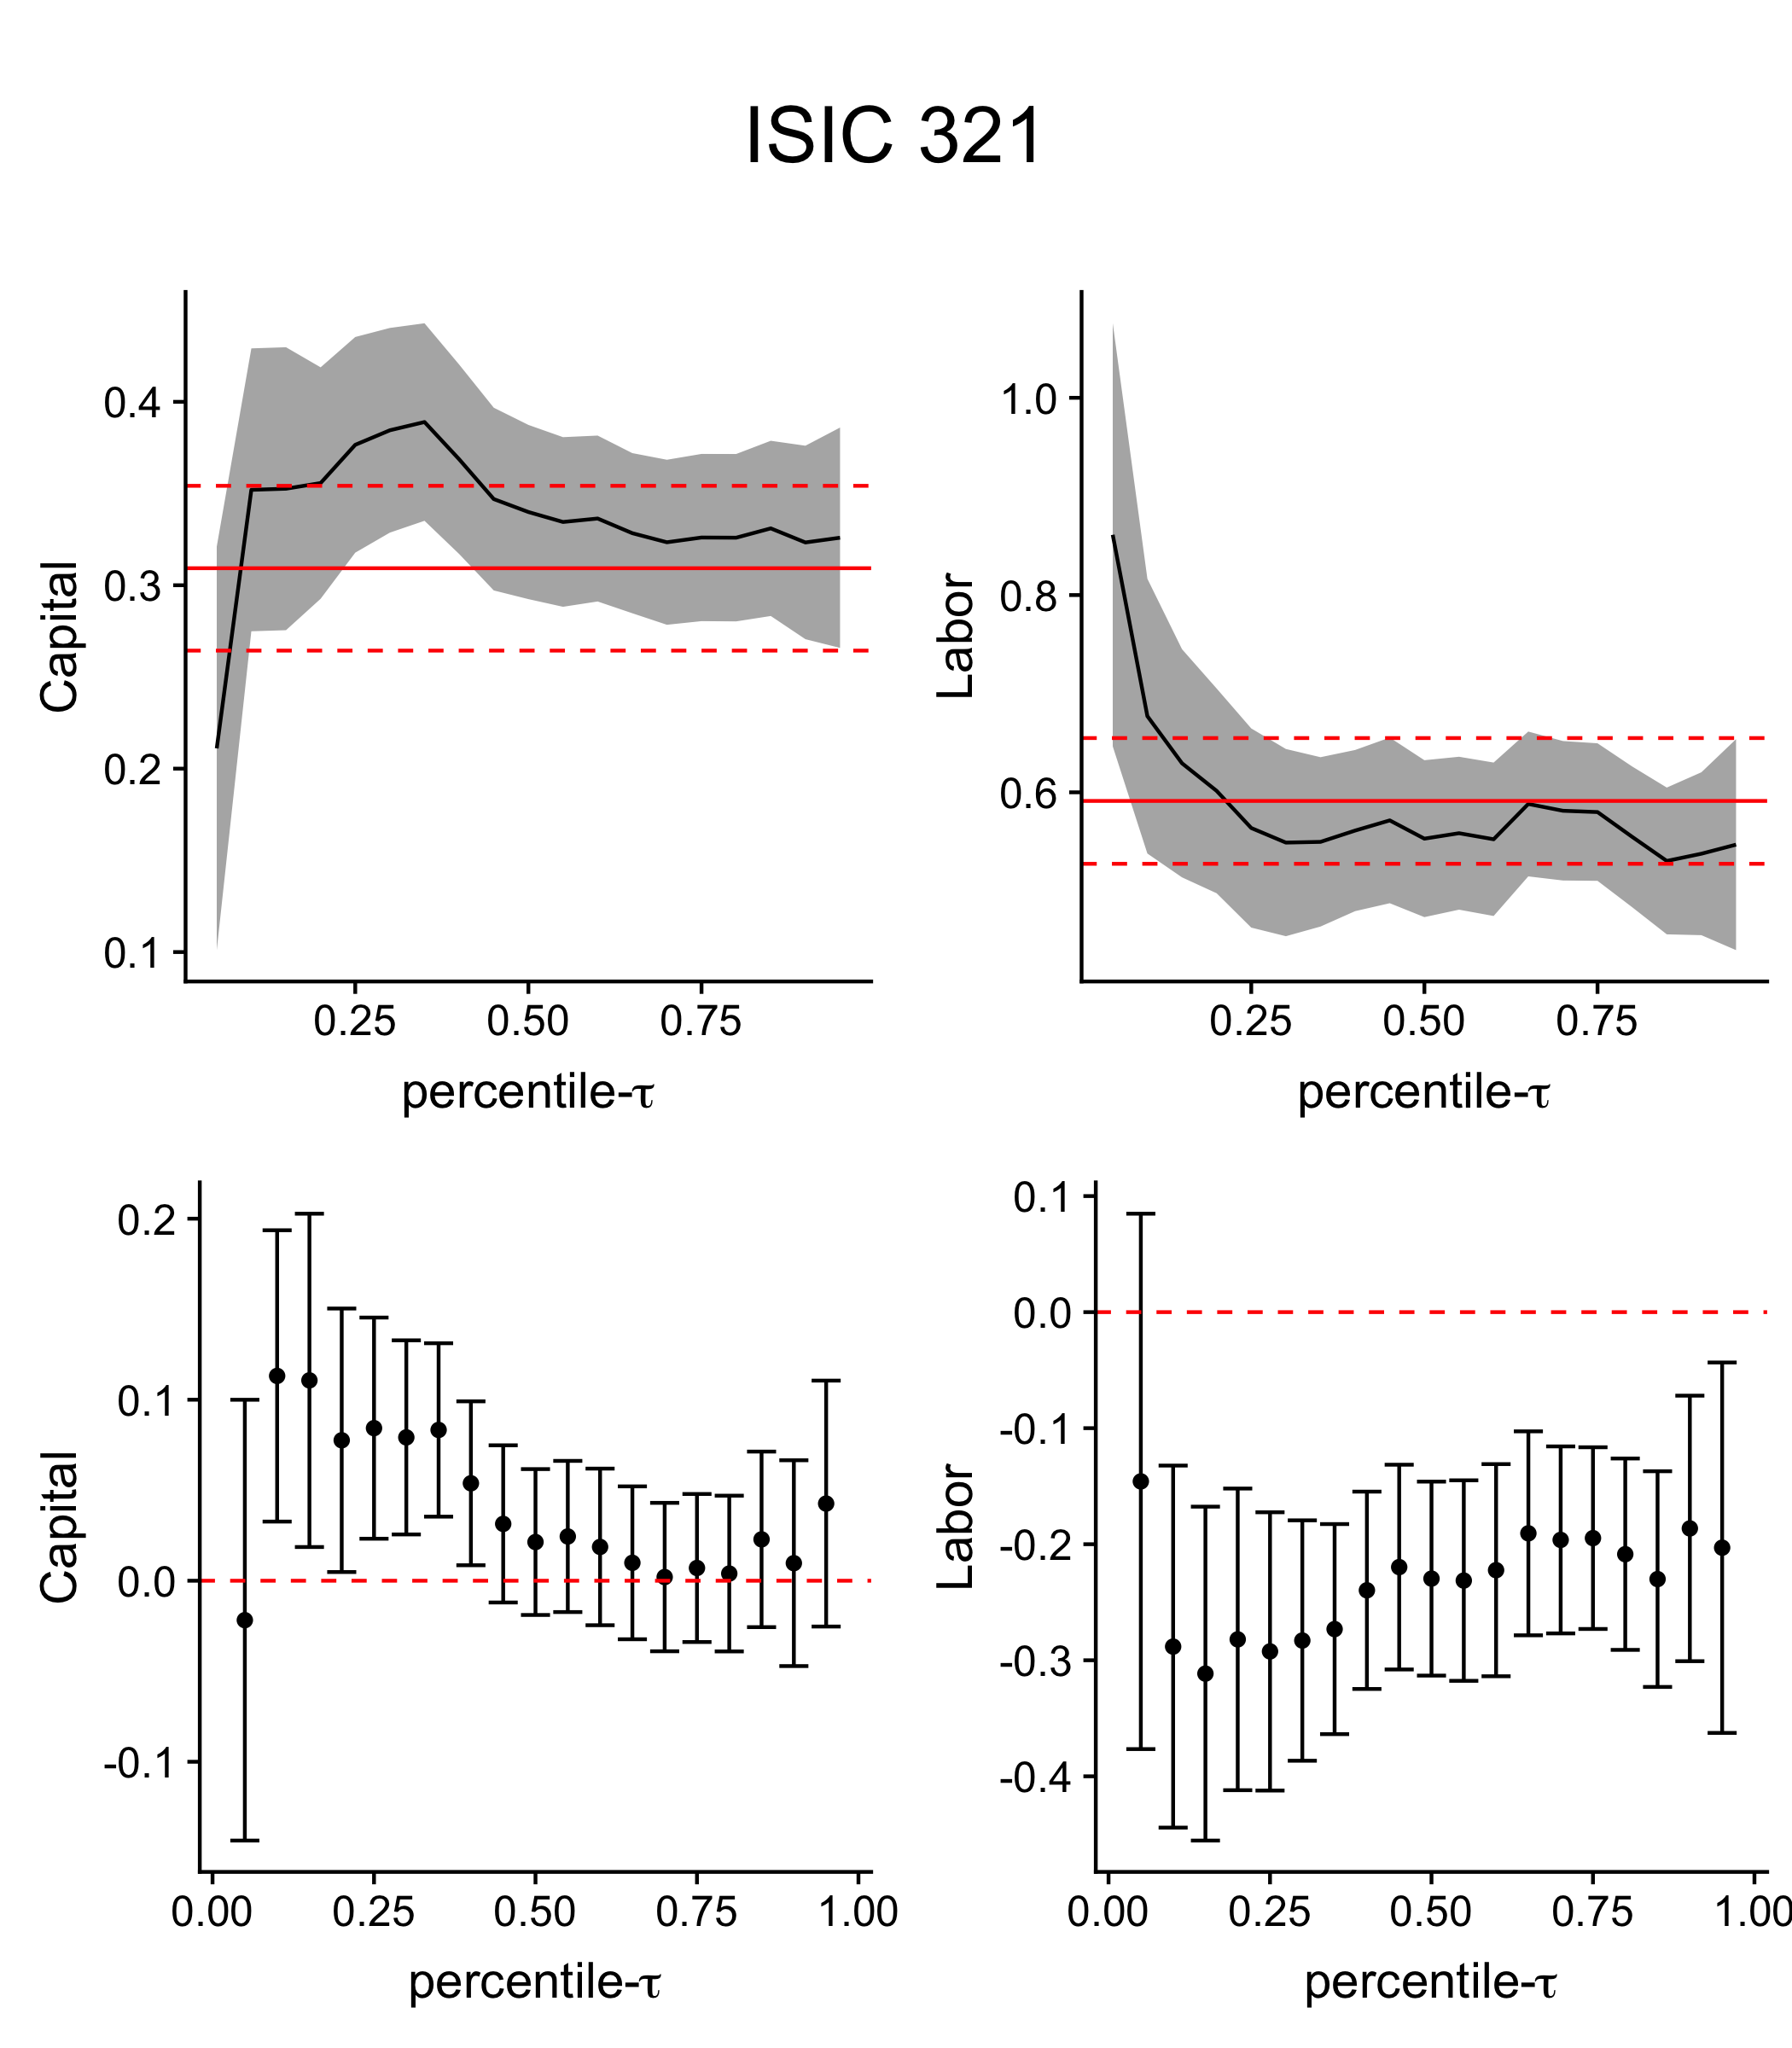
\includegraphics[width=9cm, height=9cm]{/Users/justindoty/Documents/Research/Dissertation/Production_QR_Proxy/Code/Empirical/Chile/Plots/Coef_Plot_ISIC_321.png}
\caption{Top row: Estimated values of production function coefficients and their point-wise 90\% confidence interval. Bottom row: Difference between QLP and quantile regression estimates and their 95\% confidence intervals.}
\label{fig:CHL321}
\end{figure}

\begin{figure}[H]
\centering
\includegraphics[width=9cm, height=9cm]{/Users/justindoty/Documents/Research/Dissertation/Production_QR_Proxy/Code/Empirical/Chile/Plots/Coef_Plot_ISIC_381.png}
\caption{Top row: Estimated values of production function coefficients and their point-wise 90\% confidence interval. Bottom row: Difference between QLP and quantile regression estimates and their 95\% confidence intervals.}
\label{fig:CHL381}
\end{figure}

\begin{figure}[H]
\centering
\includegraphics[width=9cm, height=9cm]{/Users/justindoty/Documents/Research/Dissertation/Production_QR_Proxy/Code/Empirical/Chile/Plots/Coef_Plot_ISIC_All.png}
\caption{Top row: Estimated values of production function coefficients and their point-wise 90\% confidence interval. Bottom row: Difference between QLP and quantile regression estimates and their 95\% confidence intervals.}
\label{fig:CHLall}
\end{figure}

% latex table generated in R 3.4.1 by xtable 1.8-2 package
% Thu Feb  4 15:46:40 2021
\begin{table}[ht]
\centering
\caption{Coefficient Estimates and Standard Errors for Chilean Manufacturing Firms} 
\begin{tabular}{cccccccccc}
  \hline\hline & & \multicolumn{2}{c}{Capital}  & \multicolumn{2}{c}{Labor} & \multicolumn{2}{c}{Returns to Scale} & \multicolumn{2}{c}{Capital Intensity}\\ \cmidrule(lr){3-4} \cmidrule(lr){5-6} \cmidrule(lr){7-8} \cmidrule(lr){9-10}ISIC & $\tau$ & Coef. & s.e & Coef. & s.e & Coef. & s.e & Coef. & s.e \\ 
  \hline
311 & 0.10 & 0.179 & 0.0248 & 0.380 & 0.0523 & 0.559 & 0.0486 & 0.470 & 0.1071 \\ 
   & 0.25 & 0.254 & 0.0246 & 0.380 & 0.0351 & 0.635 & 0.0357 & 0.668 & 0.0929 \\ 
   & 0.50 & 0.309 & 0.0232 & 0.423 & 0.0263 & 0.731 & 0.0310 & 0.730 & 0.0807 \\ 
   & 0.90 & 0.412 & 0.0248 & 0.444 & 0.0364 & 0.857 & 0.0354 & 0.927 & 0.1114 \\ 
  381 & 0.10 & 0.250 & 0.0485 & 0.774 & 0.0800 & 1.024 & 0.0570 & 0.322 & 0.1019 \\ 
   & 0.25 & 0.362 & 0.0393 & 0.649 & 0.0533 & 1.011 & 0.0460 & 0.558 & 0.1029 \\ 
   & 0.50 & 0.425 & 0.0379 & 0.606 & 0.0431 & 1.030 & 0.0405 & 0.701 & 0.1175 \\ 
   & 0.90 & 0.568 & 0.0439 & 0.503 & 0.0523 & 1.071 & 0.0450 & 1.129 & 0.2155 \\ 
  321 & 0.10 & 0.349 & 0.0571 & 0.677 & 0.0847 & 1.026 & 0.0559 & 0.516 & 0.1375 \\ 
   & 0.25 & 0.466 & 0.0478 & 0.564 & 0.0614 & 1.030 & 0.0455 & 0.827 & 0.1424 \\ 
   & 0.50 & 0.518 & 0.0440 & 0.553 & 0.0484 & 1.071 & 0.0408 & 0.937 & 0.1403 \\ 
   & 0.90 & 0.643 & 0.0481 & 0.538 & 0.0502 & 1.180 & 0.0440 & 1.195 & 0.1932 \\ 
  All & 0.10 & 0.532 & 0.0166 & 0.522 & 0.0267 & 1.055 & 0.0171 & 1.020 & 0.0799 \\ 
   & 0.25 & 0.618 & 0.0139 & 0.487 & 0.0197 & 1.105 & 0.0143 & 1.268 & 0.0725 \\ 
   & 0.50 & 0.689 & 0.0128 & 0.457 & 0.0158 & 1.145 & 0.0127 & 1.508 & 0.0720 \\ 
   & 0.90 & 0.499 & 0.0136 & 0.391 & 0.0211 & 0.891 & 0.0183 & 1.275 & 0.0935 \\ 
   \hline
\end{tabular}
\end{table}


\begin{figure}[H]
\centering
\includegraphics[width=12cm]{/Users/justindoty/Documents/Research/Dissertation/Production_QR_Proxy/Code/Empirical/Chile/Plots/TFP_Plot.png}
\caption{Estimated average productivity over time for Chile. Base productivity in 1979 is set to 100.}
\label{fig:CHLpgrowth}
\end{figure}

\begin{figure}[H]
\centering
\includegraphics[width=12cm]{/Users/justindoty/Documents/Research/Dissertation/Production_QR_Proxy/Code/Empirical/Chile/Plots/Time_Plot.png}
\caption{Estimated values of production function coefficients over time estimated at 2 year intervals}
\label{fig:CHLtimecoef}
\end{figure}


%------------------------------------------------------------------------------------------------

\subsection{Colombian Manufacturing}
This data comes from the Colombian manufacturing census conducted by the Departamento Administrativo Nacional de Estadistica. The sample is collected between 1977 and 1991. We divide our estimates into the three largest manufacturing industries: Food (ISIC 311), Apparel (ISIC 322), and Fabricated Metals (ISIC 381). As we did with the Chilean sample, we also aggregate the three industries with other smaller industries to obtain estimates from the entire sample of manufacturing plants. Summary statistics for this data is provided in Table 6.

% latex table generated in R 3.4.1 by xtable 1.8-2 package
% Wed Jan  6 11:46:20 2021
\begin{table}[H]
\centering
\caption{Summary Statistics (in logs) for Colombia Manufacturing Data} 
\begin{tabular}{ccccccc}
  \hline\hline Industry (ISIC code) &   & 1st Qu. & Median & 3rd Qu. & Mean & sd \\ 
  \hline
311 (Total=13215) & Output & 9.03 & 10.21 & 11.59 & 10.42 & 1.8 \\ 
   & Capital & 8.69 & 9.37 & 10.22 & 9.49 & 1.18 \\ 
   & Labor & 8.52 & 9.3 & 10.33 & 9.54 & 1.43 \\ 
   & Materials & 8.7 & 9.62 & 10.88 & 9.92 & 1.67 \\ 
  322 (Total=12182) & Output & 6.02 & 7.07 & 8.35 & 7.24 & 1.78 \\ 
   & Capital & 5.47 & 6.14 & 6.93 & 6.23 & 1.21 \\ 
   & Labor & 5.89 & 6.75 & 7.81 & 6.93 & 1.55 \\ 
   & Materials & 5.9 & 6.89 & 8.16 & 7.12 & 1.77 \\ 
  381 (Total=7411) & Output & 2.56 & 3.09 & 3.97 & 3.36 & 1.1 \\ 
   & Capital & 2.77 & 3.3 & 3.95 & 3.42 & 0.92 \\ 
   & Labor & 2.64 & 3.18 & 3.91 & 3.37 & 0.98 \\ 
   & Materials & 2.71 & 3.3 & 4.11 & 3.5 & 1.09 \\ 
  All (Total=87783) & Output & 8.39 & 9.73 & 11.26 & 9.87 & 2 \\ 
   & Capital & 7.62 & 8.53 & 9.46 & 8.48 & 1.51 \\ 
   & Labor & 7.77 & 8.65 & 9.72 & 8.8 & 1.58 \\ 
   & Materials & 7.89 & 8.93 & 10.26 & 9.15 & 1.88 \\ 
   \hline
\end{tabular}
\end{table}


Figures \ref{fig:COL311}, \ref{fig:COL321}, and \ref{fig:COL381} illustrate estimates from our model compared to the LP estimates as well as their differences from QR estimates. The capital estimates in each industry are increasing a significantly different than the LP estimates. The labor estimates in each industry are decreasing. In ISIC 311, 322, and the combined sample, these estimates are significantly different from LP estimates. In ISIC 381, there are only differences in the tails of the firm-size distribution. In this industry, there is also not much difference between our estimates and the QR estimates.

\begin{figure}[H]
\centering
\includegraphics[width=9cm, height=9cm]{/Users/justindoty/Documents/Research/Dissertation/Production_QR_Proxy/Code/Empirical/Colombia/Plots/Coef_Plot_ISIC_311.png}
\caption{Top row: Estimated values of production function coefficients and their point-wise 90\% confidence interval. Bottom row: Difference between QLP and quantile regression estimates and their 95\% confidence intervals.}
\label{fig:COL311}
\end{figure}

\begin{figure}[H]
\centering
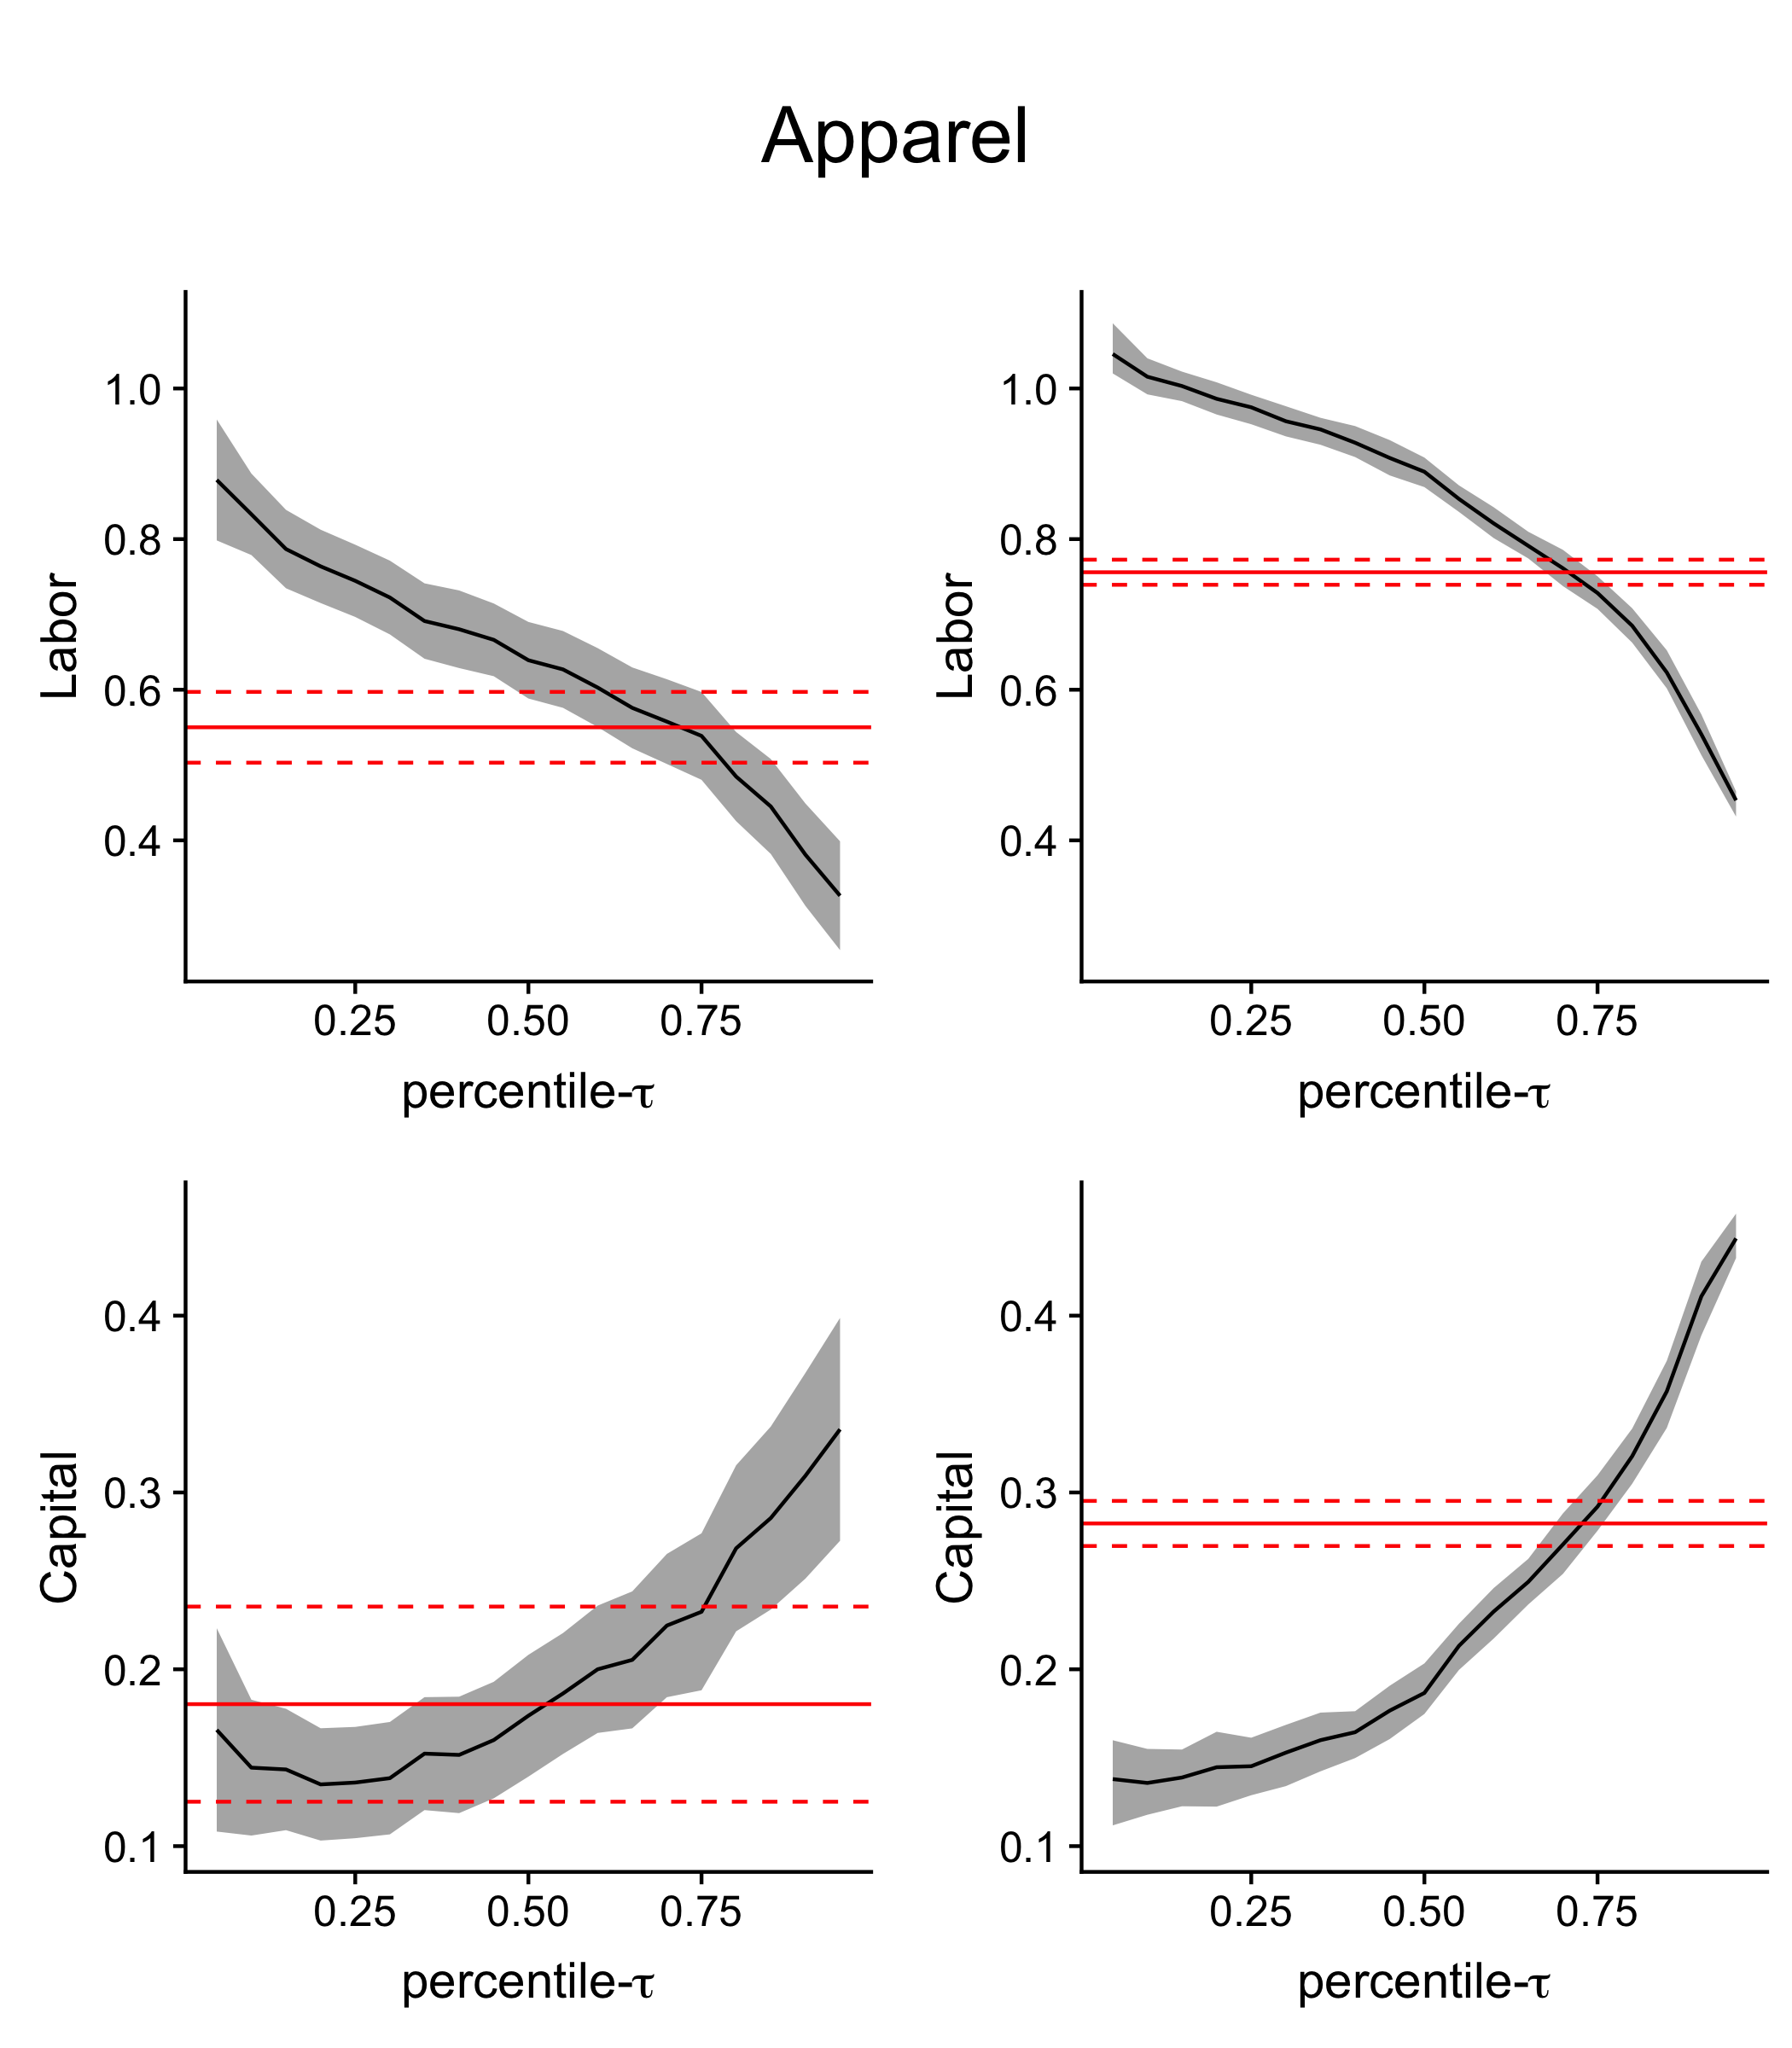
\includegraphics[width=9cm, height=9cm]{/Users/justindoty/Documents/Research/Dissertation/Production_QR_Proxy/Code/Empirical/Colombia/Plots/Coef_Plot_ISIC_322.png}
\caption{Top row: Estimated values of production function coefficients and their point-wise 90\% confidence interval. Bottom row: Difference between QLP and quantile regression estimates and their 95\% confidence intervals.}
\label{fig:COL321}
\end{figure}

\begin{figure}[H]
\centering
\includegraphics[width=9cm, height=9cm]{/Users/justindoty/Documents/Research/Dissertation/Production_QR_Proxy/Code/Empirical/Colombia/Plots/Coef_Plot_ISIC_381.png}
\caption{Top row: Estimated values of production function coefficients and their point-wise 90\% confidence interval. Bottom row: Difference between QLP and quantile regression estimates and their 95\% confidence intervals.}
\label{fig:COL381}
\end{figure}

\begin{figure}[H]
\centering
\includegraphics[width=9cm, height=9cm]{/Users/justindoty/Documents/Research/Dissertation/Production_QR_Proxy/Code/Empirical/Colombia/Plots/Coef_Plot_ISIC_All.png}
\caption{Top row: Estimated values of production function coefficients and their point-wise 90\% confidence interval. Bottom row: Difference between QLP and quantile regression estimates and their 95\% confidence intervals.}
\label{fig:COLall}
\end{figure}

Using these estimates we construct measures of returns to scale and capital intensity for each industry in Table 7. Most firms experience constant or slightly decreasing returns to scale. Returns to scale and capital intensity are increasing in firm-size.
% latex table generated in R 3.4.1 by xtable 1.8-2 package
% Wed Mar  3 23:23:10 2021
\begin{table}[ht]
\centering
\caption{Coefficient Estimates and Standard Errors for Colombian Manufacturing Firms} 
\begin{tabular}{cccccccccc}
  \hline\hline & & \multicolumn{2}{c}{Capital}  & \multicolumn{2}{c}{Labor} & \multicolumn{2}{c}{Returns to Scale} & \multicolumn{2}{c}{Capital Intensity}\\ \cmidrule(lr){3-4} \cmidrule(lr){5-6} \cmidrule(lr){7-8} \cmidrule(lr){9-10}ISIC & $\tau$ & Coef. & s.e & Coef. & s.e & Coef. & s.e & Coef. & s.e \\ 
  \hline
311 & 0.10 & 0.165 & 0.0283 & 0.641 & 0.0361 & 0.805 & 0.0361 & 0.257 & 0.0530 \\ 
   & 0.25 & 0.234 & 0.0267 & 0.619 & 0.0202 & 0.853 & 0.0300 & 0.378 & 0.0476 \\ 
   & 0.50 & 0.323 & 0.0268 & 0.532 & 0.0185 & 0.855 & 0.0293 & 0.608 & 0.0582 \\ 
   & 0.90 & 0.510 & 0.0286 & 0.350 & 0.0302 & 0.860 & 0.0326 & 1.457 & 0.1759 \\ 
  322 & 0.10 & 0.148 & 0.0246 & 0.691 & 0.0298 & 0.839 & 0.0310 & 0.214 & 0.0394 \\ 
   & 0.25 & 0.213 & 0.0253 & 0.668 & 0.0272 & 0.881 & 0.0290 & 0.319 & 0.0434 \\ 
   & 0.50 & 0.311 & 0.0259 & 0.586 & 0.0277 & 0.897 & 0.0287 & 0.530 & 0.0562 \\ 
   & 0.90 & 0.506 & 0.0332 & 0.421 & 0.0442 & 0.927 & 0.0320 & 1.203 & 0.1780 \\ 
  381 & 0.10 & 0.150 & 0.0402 & 0.952 & 0.0588 & 1.102 & 0.0529 & 0.158 & 0.0471 \\ 
   & 0.25 & 0.259 & 0.0360 & 0.872 & 0.0356 & 1.131 & 0.0450 & 0.297 & 0.0446 \\ 
   & 0.50 & 0.366 & 0.0362 & 0.762 & 0.0327 & 1.127 & 0.0434 & 0.480 & 0.0538 \\ 
   & 0.90 & 0.509 & 0.0398 & 0.661 & 0.0417 & 1.171 & 0.0436 & 0.770 & 0.0861 \\ 
  All & 0.10 & 0.091 & 0.0118 & 0.748 & 0.0146 & 0.839 & 0.0136 & 0.122 & 0.0173 \\ 
   & 0.25 & 0.178 & 0.0110 & 0.715 & 0.0104 & 0.893 & 0.0121 & 0.248 & 0.0172 \\ 
   & 0.50 & 0.263 & 0.0109 & 0.654 & 0.0090 & 0.916 & 0.0116 & 0.402 & 0.0194 \\ 
   & 0.90 & 0.410 & 0.0120 & 0.573 & 0.0125 & 0.983 & 0.0122 & 0.715 & 0.0321 \\ 
   \hline
\end{tabular}
\end{table}


Figure \ref{fig:COLpgrowth} reports average productivity for all Colombian plants in the sample with base period set to 100. Productivity decreases in the beginning of the sample period but then increases for the rest of the sample period after 1980 with some sharp periods of productivity decline and incline. Each percentile of firm-size has similar productivity levels at the beginning of the sample period, but diverge after 1984. The LP estimates show just smaller than productivity of other estimates after this time period. Figure \ref{fig:COLtimecoef} shows the time trends in output elasticities. The estimates of labor elasticity are about 0.6 for each quantile of firm-size and increases steadily until about 1981 then starts to decrease. At the end of the sample period there is more heterogeneity in these estimates. Capital estimates exhibit a clear distinction across quantiles with the larger firms having higher estimates than smaller firms. These estimates are mostly increasing until 1985 when they begin to fall.

\begin{figure}[H]
\centering
\includegraphics[width=12cm]{/Users/justindoty/Documents/Research/Dissertation/Production_QR_Proxy/Code/Empirical/Colombia/Plots/TFP_Plot.png}
\caption{Estimated average productivity over time for Colombia. Base productivity in 1978 is set to 100.}
\label{fig:COLpgrowth}
\end{figure}

% \begin{figure}[H]
% \centering
% 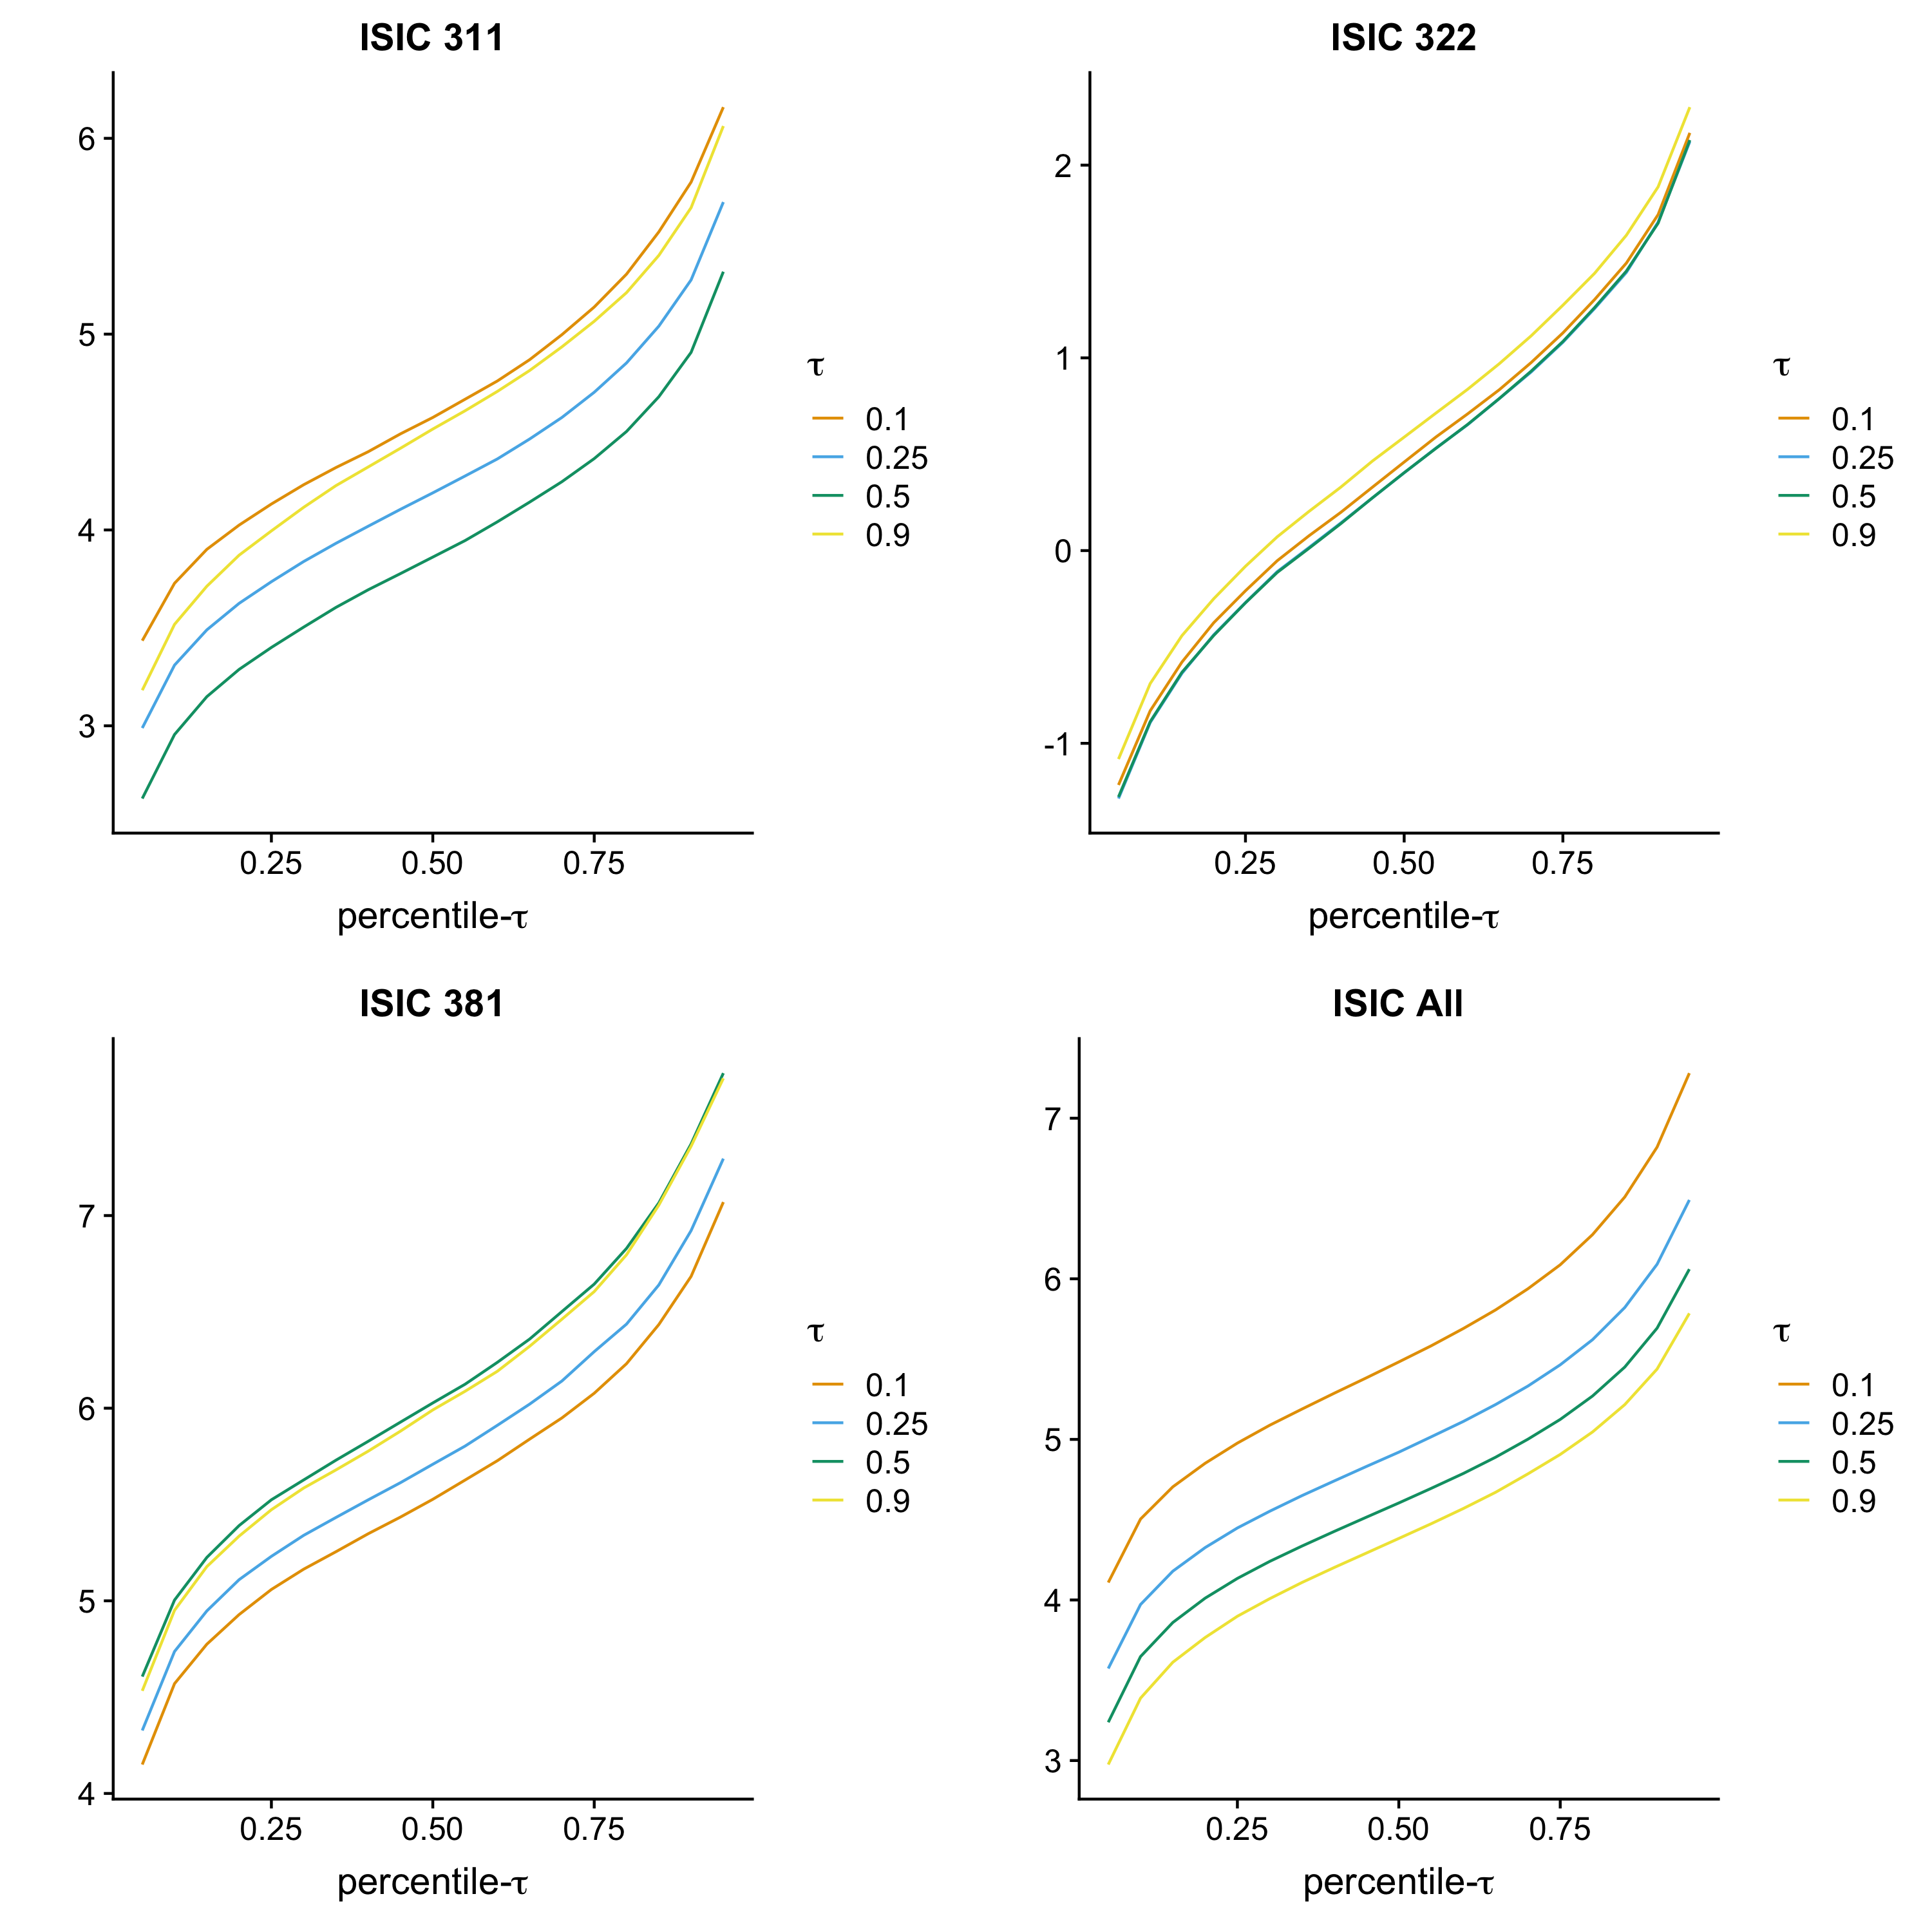
\includegraphics[width=12cm]{/Users/justindoty/Documents/Research/Dissertation/Production_QR_Proxy/Code/Empirical/Colombia/Plots/QTFP_plot.png}
% \caption{Estimated log-productivity at different quantiles over the firm-size distribution}
% \label{fig:COLpdisp}
% \end{figure}


\begin{figure}[H]
\centering
\includegraphics[width=12cm]{/Users/justindoty/Documents/Research/Dissertation/Production_QR_Proxy/Code/Empirical/Colombia/Plots/Time_Plot.png}
\caption{Estimated values of production function coefficients over time estimated at 2 year intervals}
\label{fig:COLtimecoef}
\end{figure}

\section{Conclusions} \label{conclusion}

We propose a method that extends the intermediate input proxy variable approach to estimating the conditional quantiles of firm-size. The method is computationally attractive as it resembles the two-stage estimator proposed by \cite{Canay2011}. As a result, practitioners are able to easily apply the proposed estimator to production function models where the data reveal significant heterogeneous output elasticities along the conditional firm-size distribution. We showed that this estimator works well in finite samples and showed that it captures heterogeneity in firm-size under different data generating processes. An application to widely used datasets from the US, Chile, and Colombia showed that in some industries, our estimator captures unobserved heterogeneity that the LP estimator does not.

Improvements and extensions of this estimator are currently being explored. For example, using a value-added production function may show more heterogeneity in estimates of elasticities and productivity than a gross-output production function. However, using a gross-output production function with an intermediate input proxy variable suffers from non-identification. We are currently working on an identification strategy that allows for different types of production function estimators such as the one proposed by \cite{Gandhi2020}. This paper also makes an interesting but brief connection between the literature on production risk and quantile utility maximization. Currently, quantile utility maximization problems and estimation of these models are being studied by \cite{Castro2017} and \cite{qgmm} in the context of dynamic consumption problems. It would be interesting to explore a model for a firm who maximizes quantile utility of profits which could provide an alternative interpretation for unobserved heterogeneity that are obtained from quantile regression estimates.

This paper contributes to the growing literature on production functions with unobserved heterogeneity. We show that differences in firm-size correspond to the the rank of the ex-post shock. The location-shift model for productivity we propose here restricts us from examining other dimensions of firm heterogeneity. Therefore, allowing richer distributional effects of productivity would be an interesting extension. This approach also restricts us from examining non-Hicks neutral productivity shocks such as factor-augmenting productivity. We are currently working on an extension of this paper to a non-separable model to address these last two points, but the estimator we propose here is computationally attractive and easy to implement in empirical research.    




\pagebreak
\newpage



%\section*{Appendix}
%\appendix
%\begin{Large}
%\noindent \textbf{A. Proof of the Theorems}
%\end{Large}

%\counterwithin{theorem}{section}
%\section{Proofs}





\bibliographystyle{ecca.bst}
\bibliography{references}




\end{document}